\documentclass{article}
\usepackage{iclr2027_conference,times}
\usepackage{xeCJK}
\setmainfont{texgyretermes-regular.otf}[BoldFont=texgyretermes-bold.otf,ItalicFont=texgyretermes-italic.otf,BoldItalicFont=texgyretermes-bolditalic.otf]
\setsansfont{texgyreheros-regular.otf}[BoldFont=texgyreheros-bold.otf,ItalicFont=texgyreheros-italic.otf,BoldItalicFont=texgyreheros-bolditalic.otf]
\setmonofont{texgyrecursor-regular.otf}[BoldFont=texgyrecursor-bold.otf,ItalicFont=texgyrecursor-italic.otf]
\setCJKmainfont{FandolSong-Regular.otf}[BoldFont=FandolSong-Bold.otf,ItalicFont=FandolKai-Regular.otf,SmallCapsFont=FandolSong-Regular.otf]
\setCJKsansfont{FandolHei-Regular.otf}[BoldFont=FandolHei-Bold.otf]
\setCJKmonofont{FandolFang-Regular.otf}
% Shared packages and notation. The official ICLR style is not modified.
\usepackage{amsmath,amssymb,mathrsfs}
\usepackage{microtype}
\usepackage{booktabs,array,tabularx}
\usepackage{graphicx,xcolor}
\usepackage{colortbl}
% Near-white washes; typography, rather than saturated fills, carries emphasis.
\definecolor{mainProp}{HTML}{F8FAFC}
\definecolor{mainGeneral}{HTML}{F8FBFA}
\definecolor{mainMedical}{HTML}{FDFAF8}
\definecolor{mainOurs}{HTML}{F0F4FA}
% User-selected VQA main-table palette; 3D tables retain their existing colors.
\definecolor{vqaProp}{HTML}{F6D6D6}
\definecolor{vqaGeneral}{HTML}{C0E0F8}
\definecolor{vqaMedical}{HTML}{C2E2C2}
% Table 1: retain the selected hues at 25% color on a white background.
\colorlet{vqaProp}{vqaProp!25!white}
\colorlet{vqaGeneral}{vqaGeneral!25!white}
\colorlet{vqaMedical}{vqaMedical!25!white}
% Shared by the English and Chinese manuscripts.
% Columns: PMC-VQA, VQA-RAD, SLAKE, PathVQA. Reports are in figures/report_ratescore.
% VQA: user-supplied comparison image, except Hulu-Med (Jiang et al., Table 1).
% Report values are preserved in figures/report_results.json.
% CoEvoMed-8B: user-confirmed same-checkpoint values; IU-Xray=68.22; PathVQA author-corrected to 69.40 on 2026-09-16.
% CoEvoMed-32B: six author-supplied scores on 2026-09-13; VQA-RAD corrected by author to 82.71 on 2026-09-17; report lexical metrics pending.
% A dash is unavailable, not zero.
% Qwen3.5-9B: author-supplied overall accuracy; figures/qwen35_9b_vqa_results.json.
% Qwen3-VL-8B: former Qwen3 (base) row, identity confirmed by author 2026-09-18.
% Qwen3-VL-32B: Qwen3-VL-32B-Instruct, author-supplied full metrics on 2026-09-18; 2D_result/other_model.json.
% MedVLSynther-7B: Huang et al., ICLR 2026, Table 6 (published results).
\newcommand{\MainResultsRows}{%
\midrule
\multicolumn{5}{c}{\itshape Proprietary Models}\\
\midrule
\rowcolor{vqaProp} Gemini 3 Flash & 62.62 & 69.62 & 74.55 & 52.03\\
\rowcolor{vqaProp} GPT-5.6-sol & 58.89 & 67.18 & 69.15 & 44.72\\
\rowcolor{vqaProp} Kimi-K3 & 64.48 & 73.61 & 77.13 & 53.90\\
\rowcolor{vqaProp} MiniMax-M3 & 57.33 & 68.07 & 71.44 & 57.80\\
\rowcolor{vqaProp} Qwen3.8-Max & 64.58 & 76.81 & 85.05 & 64.11\\
\midrule
\multicolumn{5}{c}{\itshape General-purpose Multimodal VLMs}\\
\midrule
\rowcolor{vqaGeneral} Qwen3-VL-8B & 54.13 & 56.76 & 64.84 & 42.77\\
\rowcolor{vqaGeneral} Qwen3.5-9B & 60.71 & 68.74 & 71.87 & 49.64\\
\rowcolor{vqaGeneral} Llama3.2-11B & 48.10 & 58.80 & 65.80 & 32.90\\
\rowcolor{vqaGeneral} InternVL3-14B & 54.10 & 66.30 & 72.80 & 48.00\\
\rowcolor{vqaGeneral} Qwen3.6-27B & 62.50 & 71.62 & 75.07 & 46.93\\
\rowcolor{vqaGeneral} Qwen3.8-27B & 60.33 & 68.51 & 73.93 & 45.11\\
\rowcolor{vqaGeneral} Qwen3-VL-32B & 57.24 & 65.85 & 71.87 & 44.28\\
\rowcolor{vqaGeneral} InternVL3-38B & 56.60 & 65.40 & 72.70 & 51.00\\
\midrule
\multicolumn{5}{c}{\itshape Medical Multimodal VLMs}\\
\midrule
\multicolumn{5}{l}{\itshape Models $<10$B}\\
\rowcolor{vqaMedical} MedGemma-4B-IT & 49.20 & 72.30 & 78.20 & 48.10\\
\rowcolor{vqaMedical} HuatuoGPT-V-7B & 53.10 & 67.60 & 68.10 & 44.80\\
\rowcolor{vqaMedical} Lingshu-7B & 56.30 & 67.90 & 83.10 & 61.90\\
\rowcolor{vqaMedical} GMAI-VL-7B & 56.09 & 57.21 & 59.69 & 39.05\\
\rowcolor{vqaMedical} MedVLSynther-7B & 55.43 & 77.57 & 72.36 & 65.56\\
\rowcolor{vqaMedical} Hulu-Med-7B & 66.80 & 78.00 & 86.80 & 65.60\\
\rowcolor{vqaMedical} \textbf{CoEvoMed (8B)} & \textbf{67.95} & \textbf{82.48} & \textbf{91.60} & \textbf{69.40}\\
\multicolumn{5}{l}{\itshape Models $>10$B}\\
\rowcolor{vqaMedical} HuatuoGPT-V-34B & 56.60 & 61.40 & 69.50 & 44.40\\
\rowcolor{vqaMedical} Lingshu-32B & 57.90 & 76.70 & 86.70 & 65.50\\
\rowcolor{vqaMedical} MedDr-40B & 13.90 & 65.20 & 66.40 & 53.50\\
\rowcolor{vqaMedical} Hulu-Med-32B & 69.40 & 81.40 & 85.70 & 67.30\\
\rowcolor{vqaMedical} \textbf{CoEvoMed (32B)} & \textbf{70.20} & \textbf{82.71} & \textbf{92.60} & \textbf{69.60}\\
\bottomrule
}

% Shared source-tagged 3D comparisons; scores scaled by 100.
\newcommand{\MThreeRows}{%
\rowcolor{mainGeneral} RadFM\textsuperscript{*} & 19.60 & 28.70 & 16.80 & 18.90 & 14.90\\
\rowcolor{mainGeneral} Qwen2.5VL-72B\textsuperscript{*} & 94.80 & 50.00 & 62.40 & 62.50 & 59.80\\
\rowcolor{mainGeneral} Lingshu-32B\textsuperscript{*} & 93.80 & 61.60 & 60.90 & 61.50 & 57.60\\
\rowcolor{mainGeneral} M3D-Llama2-7B\textsuperscript{*} & 98.80 & 79.80 & 74.80 & 66.70 & 58.90\\
\rowcolor{mainGeneral} Hulu-Med-7B\textsuperscript{*} & 99.00 & 88.00 & 78.90 & 70.70 & 67.30\\
\rowcolor{mainGeneral} Qwen3.5-9B & 96.50 & 67.25 & 59.50 & 59.06 & 57.33\\
\rowcolor{mainGeneral} Qwen3.6-27B & 96.45 & 69.95 & 63.75 & 60.84 & 59.56\\
\rowcolor{mainGeneral} Qwen3.8-27B & 95.60 & 36.55 & 63.70 & 57.92 & 56.39\\
\rowcolor{mainGeneral} Med3DVLM-7B & 99.25 & 90.65 & 80.00 & 73.28 & 66.96\\
\rowcolor{mainGeneral} Photon-3B-S1 & 51.50 & 26.50 & 42.80 & 48.73 & 48.65\\
\rowcolor{mainOurs} \textbf{CoEvoMed} & \textbf{99.50} & \textbf{91.90} & \textbf{82.20} & \textbf{73.88} & \textbf{67.80}\\
}
\newcommand{\RadThreeRows}{%
\rowcolor{mainGeneral} Qwen2.5VL-72B\textsuperscript{*} & 15.50 & 25.20 & 16.90 & 27.30 & 6.70 & 11.60\\
\rowcolor{mainGeneral} M3D (Phi3-4B)\textsuperscript{*} & 16.30 & 23.20 & 15.10 & 23.20 & 2.50 & 5.60\\
\rowcolor{mainGeneral} Lingshu-7B\textsuperscript{*} & 9.30 & 21.60 & 10.40 & 22.20 & 0.90 & 8.40\\
\rowcolor{mainGeneral} M3D (Llama2-7B)\textsuperscript{*} & 10.70 & 20.80 & 9.10 & 18.60 & 15.90 & 23.20\\
\rowcolor{mainGeneral} Lingshu-32B\textsuperscript{*} & 7.60 & 16.10 & 7.80 & 16.30 & 0.90 & 4.80\\
\rowcolor{mainGeneral} Hulu-Med-7B\textsuperscript{*} & 23.40 & 35.90 & 23.00 & 37.10 & 23.50 & 26.00\\
\rowcolor{mainGeneral} Qwen3.5-9B & 12.85 & 25.04 & 14.07 & 24.18 & 7.05 & 15.17\\
\rowcolor{mainGeneral} Qwen3.6-27B & 22.47 & 29.68 & 23.09 & 30.76 & 2.89 & 7.99\\
\rowcolor{mainGeneral} Qwen3.8-27B & 12.70 & 26.63 & 14.62 & 30.00 & 13.08 & 13.77\\
\rowcolor{mainGeneral} Med3DVLM-7B & 0.68 & 6.23 & 0.77 & 5.79 & 0.11 & 0.46\\
\rowcolor{mainGeneral} Photon-3B-S2 (local) & 37.93 & 37.58 & 48.09 & 47.26 & 29.22 & 31.13\\
\rowcolor{mainOurs} \textbf{CoEvoMed} & \textbf{38.60} & \textbf{44.86} & \textbf{52.36} & \textbf{57.06} & \textbf{37.83} & \textbf{39.30}\\
}
\newcommand{\AmossRows}{%
\rowcolor{mainGeneral} Qwen3.6-27B & 46.44 & 15.49 & 18.88 & 13.16\\
\rowcolor{mainGeneral} Hulu-Med-7B & 64.35 & 35.84 & 37.49 & 30.51\\
\rowcolor{mainGeneral} M3D-Llama3.1-8B\textsuperscript{*} & 57.00 & 26.40 & 37.90 & \textbf{35.50}\\
\rowcolor{mainGeneral} M3D-Mistralv0.3-7B\textsuperscript{*} & 56.90 & 25.80 & 37.40 & 34.60\\
\rowcolor{mainGeneral} Qwen2.5VL-32B\textsuperscript{*} & 52.90 & 24.60 & 19.10 & 21.10\\
\rowcolor{mainGeneral} Qwen3.5-9B & 53.68 & 29.26 & 21.40 & 20.04\\
\rowcolor{mainGeneral} Qwen3.8-27B & 50.02 & 23.06 & 18.93 & 16.34\\
\rowcolor{mainGeneral} Med3DVLM-7B & 42.84 & 11.63 & 15.66 & 10.34\\
\rowcolor{mainGeneral} Lingshu-7B & 50.75 & 24.43 & 19.89 & 17.75\\
\rowcolor{mainGeneral} Lingshu-32B & 45.22 & 24.45 & 17.43 & 16.75\\
\rowcolor{mainGeneral} M3D-LaMed-4B & 39.00 & 4.32 & 12.57 & 5.87\\
\rowcolor{mainOurs} \textbf{CoEvoMed} & \textbf{66.97} & \textbf{39.30} & \textbf{40.40} & 31.91\\
}

\usepackage{tikz}
\usetikzlibrary{arrows.meta,positioning,fit,backgrounds}
\usepackage{placeins}
\usepackage{float}
% Pseudocode uses the existing float/tabularx packages; captions remain below.
\floatstyle{plain}
\newfloat{algorithm}{htbp}{loa}
\floatname{algorithm}{Algorithm}
\usepackage{wrapfig}
% Keep natural vertical spacing when an indivisible table moves to the next page.
% Do not stretch headings and paragraph gaps to force page-bottom alignment.
\AtBeginDocument{\raggedbottom}
\usepackage{hyperref}
% Allow long reference URLs to wrap without stretching the surrounding words.
\usepackage{xurl}
\hypersetup{colorlinks=true,linkcolor=blue!45!black,citecolor=blue!45!black,urlcolor=blue!45!black,pdfauthor={Anonymous authors}}
\newcommand{\tbd}{\textcolor{black!65}{\textsf{TBD}}}
\newcommand{\obs}{o}
\newcommand{\hist}{h}
\newcommand{\strategies}{\Sigma}
\newcommand{\evol}{\mathscr E}
\newcommand{\cellset}{\mathcal C}
\newcommand{\source}{\mathcal S}
\newcommand{\trainset}{\mathcal D}
\newcommand{\E}{\mathbb E}
\newcommand{\ind}{\mathbf 1}
\newcolumntype{L}[1]{>{\raggedright\arraybackslash}p{#1}}
\newcolumntype{Y}{>{\raggedright\arraybackslash}X}

% Language-specific labels are supplied by each main file.
\newcommand{\frameworkfigure}{%
\begin{tikzpicture}[
  box/.style={draw=black!60,rounded corners=2pt,align=center,font=\small,
    minimum height=0.80cm,text width=3.45cm,inner sep=4pt},
  arrow/.style={-{Latex[length=2mm]},thick,draw=black!70},
  feed/.style={arrow,dashed},node distance=0.7cm and 0.6cm]
  \node[box,fill=blue!6] (feedback) {\FigFeedback};
  \node[box,fill=blue!6,right=of feedback] (policy) {\FigPolicy};
  \node[box,fill=orange!9,right=of policy] (synth) {\FigSynthesis};
  \node[box,fill=orange!9,below=of synth] (student) {\FigStudent};
  \node[box,fill=orange!9,left=of student] (strategy) {\FigStrategy};
  \node[box,fill=black!3,left=of strategy] (record) {\FigRecord};
  \draw[arrow] (feedback) -- (policy);
  \draw[arrow] (policy) -- (synth);
  \draw[arrow] (synth) -- (student);
  \draw[arrow] (student.south) -- ++(0,-0.45) -| (record.south);
  \draw[arrow] (record) -- (feedback);
  \draw[feed] (feedback.south) -- (strategy.north west);
  \draw[arrow] (strategy.north east) -- (synth.south west);
\end{tikzpicture}%
}

% An honest placeholder for future measurements, not an illustrative result curve.
\newcommand{\trajectoryplaceholder}{%
\begin{tikzpicture}[font=\small]
  \draw[draw=black!45,rounded corners=2pt] (0,2.5) rectangle (12.8,4.6);
  \node at (6.4,4.1) {\FigCapability};
  \node[align=center,text width=11.5cm,text=black!60] at (6.4,3.25) {\FigPending};
  \draw[draw=black!45,rounded corners=2pt] (0,0) rectangle (6.2,2.2);
  \draw[draw=black!45,rounded corners=2pt] (6.6,0) rectangle (12.8,2.2);
  \node at (3.1,1.7) {\FigVQA};
  \node at (9.7,1.7) {\FigReport};
  \node[align=center,text width=5.5cm,text=black!60] at (3.1,0.9) {\FigPending};
  \node[align=center,text width=5.5cm,text=black!60] at (9.7,0.9) {\FigPending};
\end{tikzpicture}%
}

\title{CoEvoMed: Co-Evolving Supervision Principles and Medical Vision--Language Models}
\hypersetup{pdftitle={CoEvoMed: Co-Evolving Supervision Principles and Medical Vision–Language Models}}
\author{Anonymous Authors}
% 中文阅读稿；保留官方匿名审稿样式，不启用 \iclrfinalcopy。
\newcommand{\FigFeedback}{任务验证集 $\mathcal V$\\学习动态与课程需求}
\newcommand{\FigPolicy}{课程适配\\修复、保持与弱点聚焦}
\newcommand{\FigSynthesis}{多智能体协作\\证据约束的监督构造}
\newcommand{\FigStudent}{学习者更新\\$M_e\longrightarrow M_{e+1}$}
\newcommand{\FigStrategy}{监督构造原则\\学习响应驱动的演化}
\newcommand{\FigRecord}{能力发展\\$\widehat{\boldsymbol\kappa}_e\longrightarrow\widehat{\boldsymbol\kappa}_{e+1}$}
\newcommand{\FigExternal}{运行结束后外部测试\\$\mathcal B_{\mathrm{ext}}$}
\newcommand{\FigVQA}{外部 VQA 基准}
\newcommand{\FigReport}{外部描述／报告测试}
\newcommand{\FigPending}{CoEvoMed 与静态合成\\实测数据：TBD}
\newcommand{\FigCapability}{任务验证上的能力轨迹}
\begin{document}
\maketitle
\begin{abstract}
医学视觉语言模型训练需要训练监督能够适应学习者在不同任务上不断变化的能力。现有流程通常依赖反复的人工错误分析和面向任务的训练数据构建，使这一适应过程成本高昂。我们提出共演化框架 CoEvoMed，将医学视觉语言学习者与融合构造原则演化和课程分配的多智能体监督过程相耦合。这些可复用的原则明确问题意图，指导回答如何依据医学证据形成，并厘清训练样本中的概念区别。原则修订智能体根据学习者在不同任务上不断变化的能力更新这些原则，并通过比较基于相同医学证据生成的样本在事实一致性与任务契合度上的表现来指导修订。在各任务预算固定的条件下，课程分配根据学习者的能力表现与学习进展调整构造投入。借助 CoEvoMed，我们训练了一个同时支持 2D 与 3D 医学任务的 8B 模型。该模型在四项 2D VQA 基准上较 Hulu-Med-7B 提升 1.15--4.80 个百分点，在 MIMIC-CXR 与 IU-Xray 上取得更高的 RaTEScore，并在三维识别、问答与报告生成任务上表现出较强能力。32B 实验进一步支持了该框架的规模可扩展性。
\end{abstract}
\begin{figure}[H]
\centering
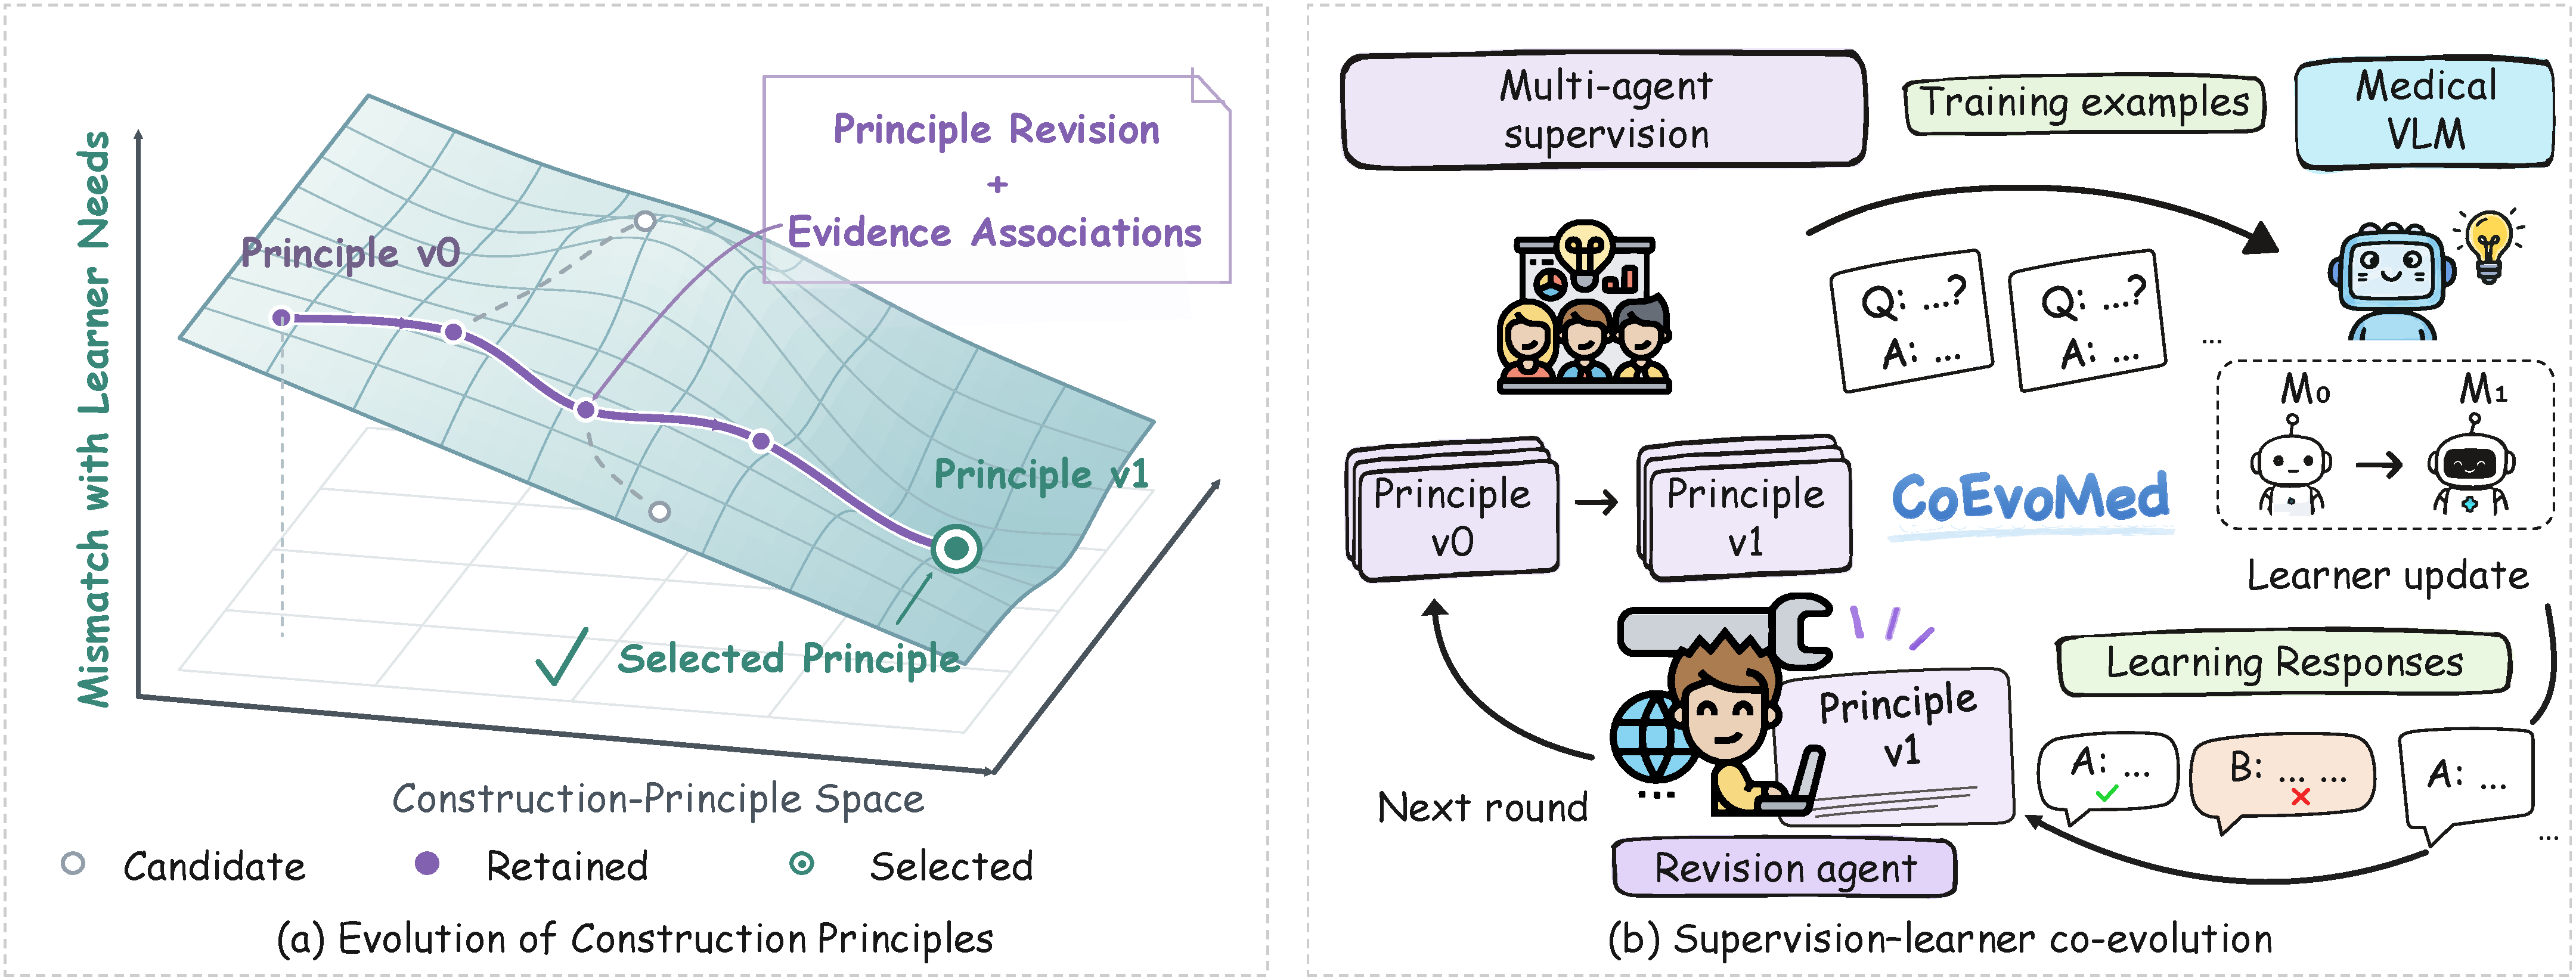
\includegraphics[width=\linewidth]{figures/evoforma_concept.pdf}
\caption{CoEvoMed 的共演化机制。（a）学习响应引导原则演化。（b）多智能体过程连接监督构造、学习者更新与原则修订。}
\label{fig:concept}
\end{figure}
\FloatBarrier
\section{引言}
\label{sec:intro}

训练数据所覆盖的知识及其监督组织方式，是医学多模态模型能力形成的重要约束。前者界定可供学习的医学证据范围，后者组织模型从这些证据中学习的任务目标与推理关系。监督的有效性依赖于其与学习者当前状态的匹配程度。随着训练推进，模型在不同任务上的掌握程度与学习收益持续分化，预先固定的监督组织方式因而难以维持对后续能力发展的适配性。医学多模态学习由此要求将数据构建视为训练过程的内生组成，使监督构造与训练分配随学习者的发展持续调整。

现有的数据迭代实践通常依赖人工检视错误与归纳失效模式~\citep{wu2019errudite}，并据此定向构造监督~\citep{khan2025dataenvgym}。此类流程需要反复开展细粒度诊断和监督设计，具有较高的人力成本~\citep{ribeiro2022adaptive}，且难以将持续变化的学习需求及时转化为系统性的训练干预。这一局限推动了从静态监督供给向学习响应驱动的监督构造的转变：以观测到的学习响应修订可复用的监督构造原则，并以实际学习增益调节训练资源分配，使监督构造与模型学习形成相互驱动的演化过程。

课程学习适应性地选择内容并分配资源~\citep{bengio2009curriculum,matiisen2017teacher}；DataEnvGym 利用学生反馈迭代生成数据~\citep{khan2025dataenvgym}；Evo-PI 演化医学推理评价与奖励原则~\citep{zheng2026evopi}。本文关注构造原则与学习者能力的双向发展：学习响应修订证据的监督表达，修订后的监督塑造后续学习，将监督构造的演化与有限构造资源的配置相联系。

我们提出 \emph{CoEvoMed}，以\emph{学习响应驱动的监督构造}实现监督构造智能体与多模态学习者的共演化。可复用构造原则规定提问意图、证据关联与概念辨析；任务级能力状态评估引导原则演化与后续监督适配，残余错误进一步指导原则修订，实际学习增益调节固定预算下不同能力的构造投入。多智能体在匹配证据与目标下比较候选原则，评价监督适配性与事实一致性。选定原则塑造后续监督，所得学习响应引导进一步修订。按任务组织的独立验证集提供响应，共享支持集承载构造所依据的医学证据，独立外部基准评价学习结果。构造原则的演化与学习者能力的发展共同塑造学习轨迹。

本文的主要贡献概括如下：

\noindent\textbullet\enspace 我们提出一个共演化框架，将构造原则的演化纳入学习者训练，通过双向反馈将监督构造与能力发展相联系。

\noindent\textbullet\enspace 我们设计课程分配策略，平衡较弱能力的提升与已掌握能力的保持。随着学习者能力发展，学习进展指导固定构造预算的重新分配。

\noindent\textbullet\enspace 我们构建多智能体系统，整合课程分配与原则演化。课程分配引导不同能力的监督构造投入，持续演化的原则指导如何将医学证据组织为训练样本。


\section{相关工作}
\label{sec:related}

\subsection{课程学习与自适应监督}

课程学习依据样本难度组织训练~\citep{bengio2009curriculum}，自适应教学则根据学习进展或学习者状态选择样本~\citep{matiisen2017teacher,liu2017iterative}。研究进一步从样本选择拓展至监督构造：Generative Teaching Networks 通过元梯度优化合成监督~\citep{such2020generative}，DataEnvGym 利用学习者反馈引导数据生成~\citep{khan2025dataenvgym}。近期方法将任务生成、视觉监督或任务知识与学习者的发展相耦合~\citep{huang2026rzero,zhang2026viper,wu2026k2}。CoEvoMed 联合调整监督构造与课程分配：可复用构造原则随学习响应演化，实际学习增益则引导不同能力之间的构造投入。

\subsection{多智能体适应与共演化}

Self-Instruct 生成指令跟随监督~\citep{wang2023self}。AutoGen 组织智能体对话~\citep{wu2024autogen}，Graph-of-Agents 根据任务调整协作结构~\citep{yun2026graph}。Automated Design of Agentic Systems 通过元智能体搜索智能体程序~\citep{hu2025automated}。反馈也支持不同层面的适应：Self-Refine 修订输出~\citep{madaan2023selfrefine}，Reflexion 在多次尝试之间保留语言化反思~\citep{shinn2023reflexion}，ACE 完善上下文~\citep{zhang2026agentic}。CoMAS 利用交互奖励优化参与智能体的策略~\citep{xue2026comas}。CoEvoMed 研究跨越监督构造与多模态学习的共演化：智能体依据学习者的发展修订证据约束的构造原则，这些原则所诱导的监督则塑造后续学习。

\subsection{医学多模态学习}

医学视觉语言任务覆盖放射学、病理学、文献图像问答及报告生成~\citep{lau2018dataset,liu2021slake,he2020pathvqa,zhang2024pmc,johnson2019mimic,demnerfushman2016preparing}。LLaVA-Med 与 Med-Flamingo 分别研究生物医学指令训练和少样本适应~\citep{li2023llava,moor2023med}。RadFM 将文本与二维、三维放射影像输入相结合~\citep{wu2025radfm}，M3D 则构建面向三维医学任务的体积影像--文本及指令数据~\citep{bai2024m3d}。MedVLSynther 提出源条件生成与规则化验证~\citep{huang2026synthesizing}，MMedAgent-RL 引入面向协作的专科可靠性课程~\citep{xia2026mmedagent}。CoEvoMed 在不同视觉场景与骨干家族中研究适应学习者能力的监督构造。

\section{问题定义}
\label{sec:problem}

本文对构造原则与学习者能力的共演化进行形式化描述，并将其中的课程分配建模为序贯决策问题。在第 $e$ 轮，分配向量 $\boldsymbol q_e$ 规定有限构造预算在各任务内预先定义的能力单元之间的分配比例，并满足固定的任务级配额约束。构造原则 $\Sigma_e$ 是决定如何将医学证据组织为面向目标能力的监督的可复用规范。这些原则明确问题意图，指导回答如何依据医学证据形成，并厘清概念区别。

\subsection{学习者状态与课程分配}

第$e$轮的学习者$M_e$在独立任务验证集$\mathcal V=\{\mathcal V_t\}_{t\in\mathcal T}$上接受评价，其中$\mathcal T$为验证任务集合。支持集$\mathcal S$提供监督构造所需的医学视觉证据及关联文本，独立外部基准评价泛化。预先定义的能力单元组成$\mathcal C$，每个单元$c$在固定非空子集$\mathcal V_c\subseteq\mathcal V_t$上接受评价。能力评价泛函$\mathcal J_c$将预测行为映射为实测掌握水平：
\begin{equation}
\mathcal J_c[M_e]=\frac{1}{|\mathcal V_c|}\sum_{z\in\mathcal V_c}u_c(M_e,z),
\qquad
\widehat{\boldsymbol\kappa}_e=\bigl(\mathcal J_c[M_e]\bigr)_{c\in\mathcal C}.
\label{eq:capability_level}
\end{equation}
其中，$u_c$为对每个样本赋予分数的固定评价规则，分数越高表示表现越好。向量$\widehat{\boldsymbol\kappa}_e$为可观测能力表征。任务表现与错误证据共同构成观测$o_e$。

课程规划器依据历史摘要$\mathbf{s}_e=\Phi(h_e)$选择课程动作$a_e$，其中$h_e$记录截至第$e$轮的观测、动作与奖励。我们以有限时域部分可观测马尔可夫决策过程刻画这一交互~\citep{kaelbling1998planning,matiisen2017teacher}。完整状态$X_e$包含学习者参数与优化状态、生效构造原则、修订历史、调度信息及剩余资源。给定原则演化规则$\mathscr E$，有
\begin{equation}
P(X_{e+1}\mid X_{0:e},a_{0:e})
=P_{\mathscr E}(X_{e+1}\mid X_e,a_e).
\label{eq:transition}
\end{equation}
转移包括监督构造、验证、学习者更新及学习响应驱动的原则修订。附录~\ref{app:formalization}给出完整状态与观测模型。

\subsection{监督构造}
\label{sec:supervision_evolution}

对于由视觉输入、指令与目标回答组成的$z=(v,x,y)$，候选训练样本的分布为
\begin{equation}
\widetilde p_e(z)=\sum_{c\in\mathcal C}q_{e,c}\,
g_{e,c}(z;\Sigma_e,\mathcal S).
\label{eq:supervision_mixture}
\end{equation}
其中，$g_{e,c}$表示第$e$轮面向能力单元$c$的候选训练样本在验证前的概率分布，由构造原则$\Sigma_e$指导、利用支持集$\mathcal S$开展的证据选择与监督构造过程诱导。非负份额$q_{e,c}$的总和为1。原则演化改变各分量的监督内容，课程分配改变其相对投入。证据约束的验证形成接受的监督$\mathcal D_e^{\mathrm{syn}}$，后续混合确定实际训练曝光。

\subsection{学习者更新与策略目标}

训练混合数据$\mathcal D_e^{\mathrm{mix}}$由已接受的监督$\mathcal D_e^{\mathrm{syn}}$与允许使用且仅用于训练的原始或回放数据$\mathcal R_e$组成。学习者更新为
\begin{equation}
M_{e+1}=\mathcal U(M_e,\mathcal D_e^{\mathrm{mix}}),
\label{eq:learning_dynamics}
\end{equation}
其中，$\mathcal U$遵循规定训练协议及优化状态。各轮能力表征记录$E$轮训练中的学习者能力发展。$M_{e+1}$的响应进入$h_{e+1}$，并通过式~\ref{eq:strategy_evolution}修订$\Sigma_{e+1}$，将原则演化与后续学习相联系。

在这一动态中，分配策略最大化累积验证学习进展：
\begin{equation}
\max_{\pi\in\Pi_{\mathrm{adm}}}
\E_{\pi}\left[\sum_{e=0}^{E-1}\gamma^e r_e\right],
\label{eq:objective}
\end{equation}
其中，$\Pi_{\mathrm{adm}}$表示满足构造预算约束并保持各任务规定配额的课程分配策略集合，$\gamma\in[0,1]$为折扣因子。奖励$r_e$衡量对 VQA 与报告生成赋予相同权重的验证表现增益（第~\ref{sec:curriculum}节）。附录~\ref{app:cumulative_gains}给出累积增益与各轮学习表现之间的关系。

\FloatBarrier

\section{CoEvoMed：监督构造智能体与多模态学习者的共演化}
\label{sec:method}

\begingroup
\setlength{\intextsep}{2pt}
\begin{figure}[H]
\centering
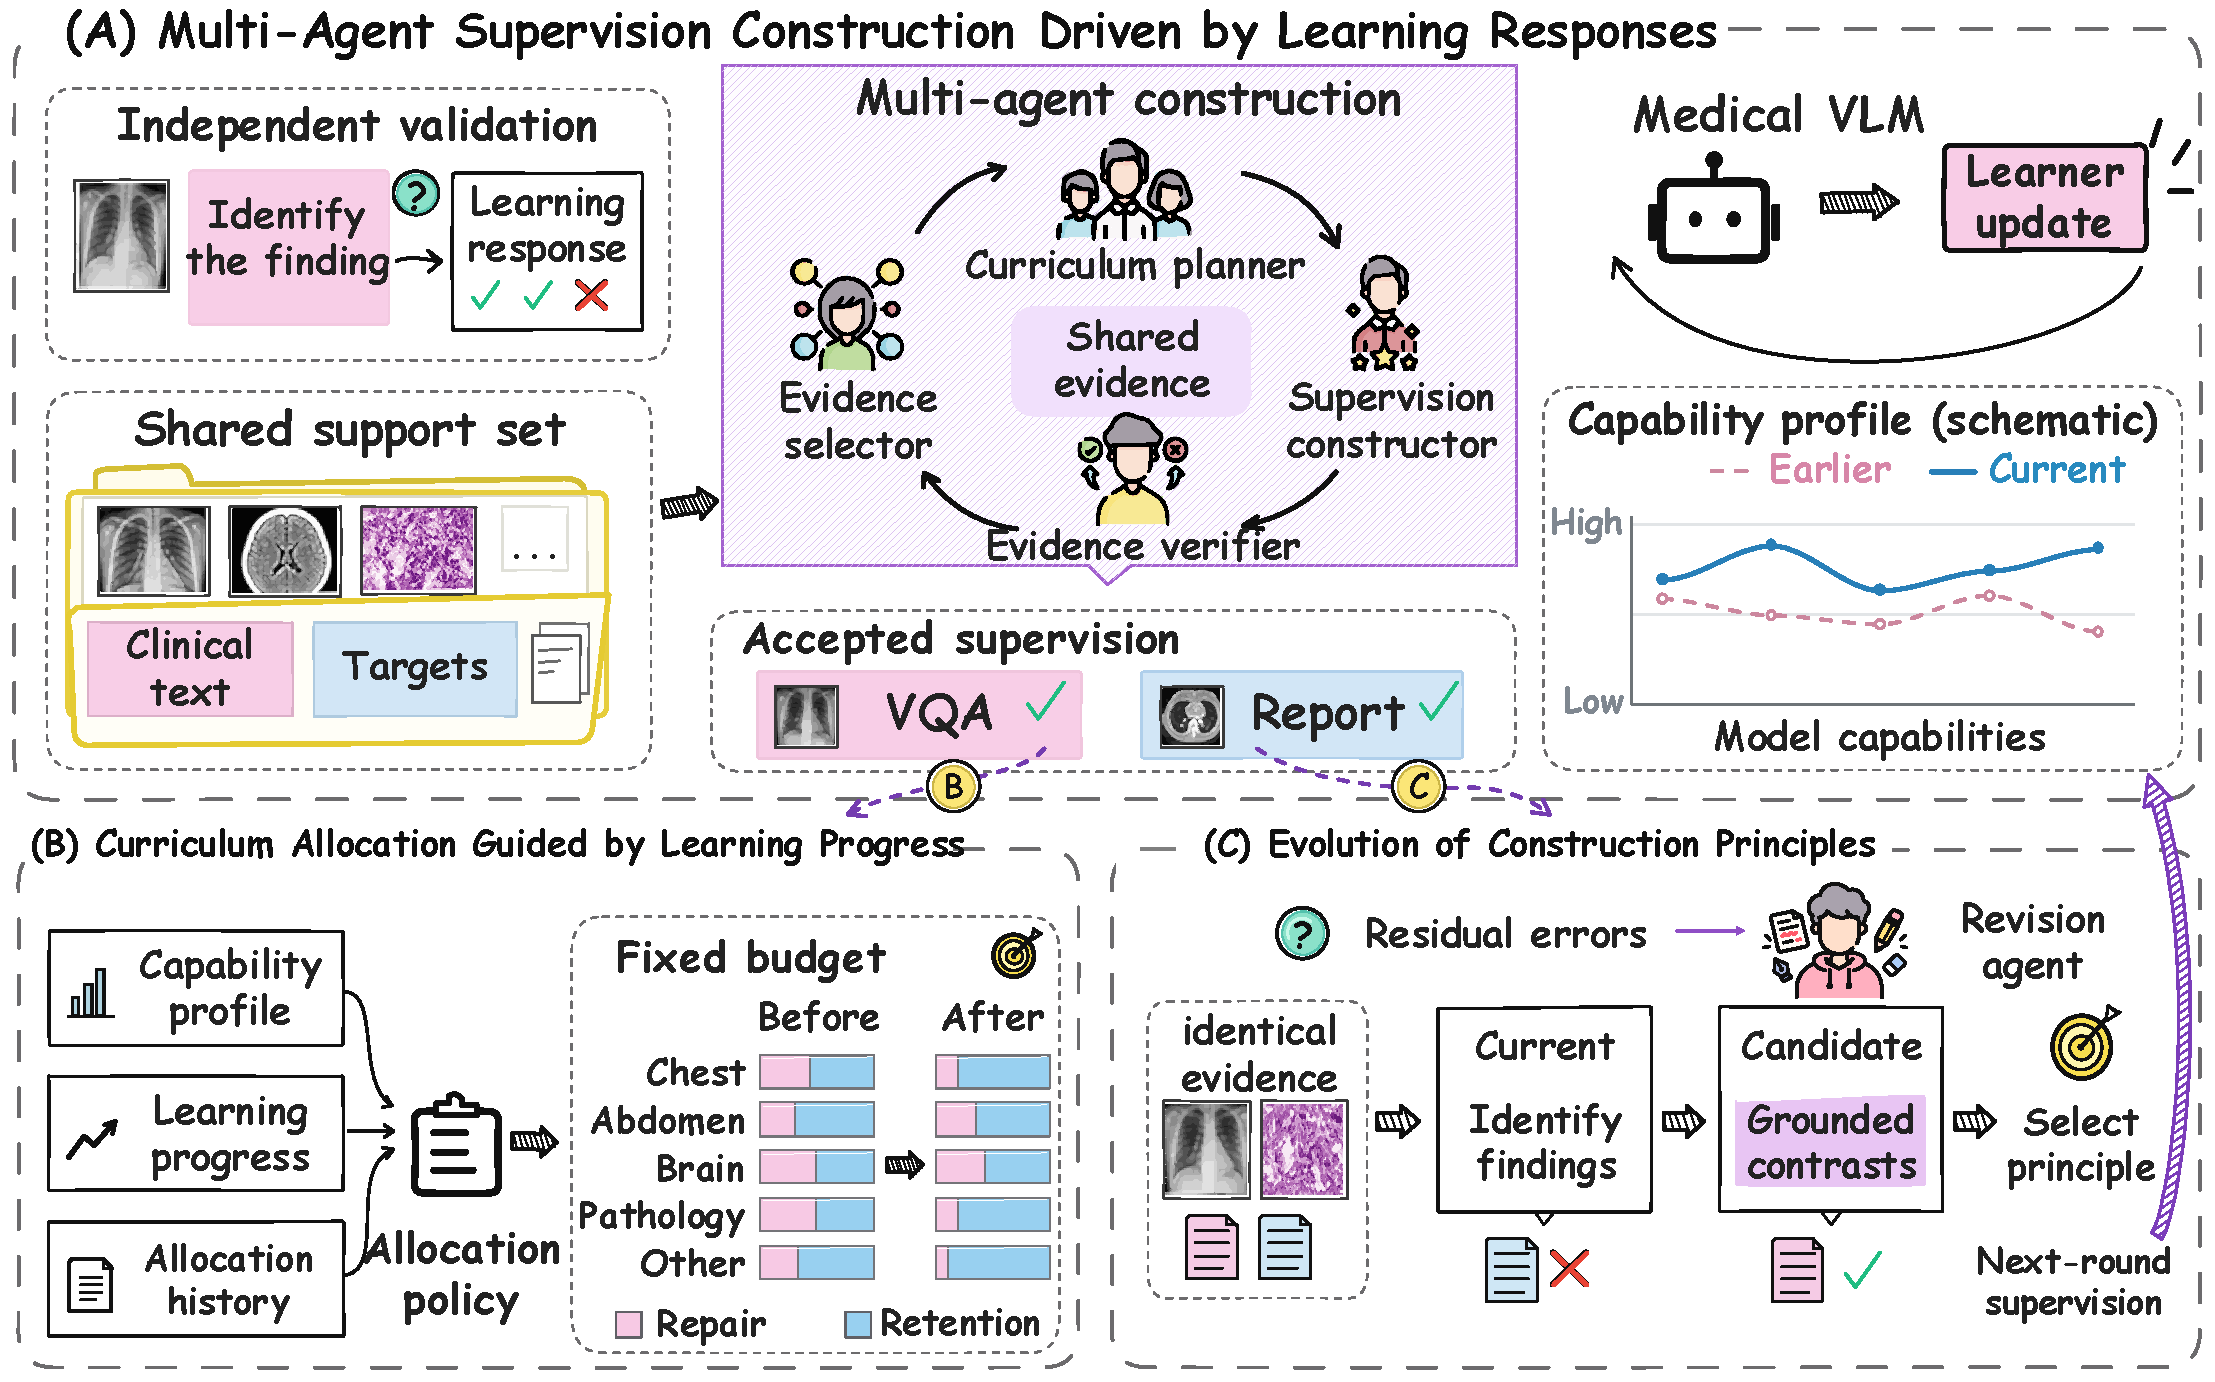
\includegraphics[width=\linewidth]{figures/evoforma_framework.pdf}
\caption{CoEvoMed 框架。（A）多智能体协作基于医学证据构造并验证监督，学习者更新后在独立任务验证集上产生学习响应。（B）学习进展指导固定任务预算下的课程分配。（C）修订智能体依据学习响应修订构造原则，比较当前原则与候选原则基于相同证据生成的监督；被接受的修订用于后续监督构造。}
\label{fig:framework}
\end{figure}
\endgroup

CoEvoMed 通过学习响应将监督构造与学习者更新联系起来（图~\ref{fig:framework}）。其多智能体系统结合课程分配与原则演化：课程分配决定构造投入，修订后的原则则改变智能体将医学证据组织为监督的方式。

\subsection{学习响应驱动的多智能体监督构造}
\label{sec:multiagent}

课程规划器依据能力反馈确定分配份额与构造目标。证据选择器从$\mathcal S$检索兼容的视觉记录与支持事实；监督构造器依据$\Sigma_e$形成问答对或报告，证据验证器检查事实一致性、视觉依赖、有效性与重复。接受的监督$\mathcal D_e^{\mathrm{syn}}$保留其证据来源与所用原则，用于后续评价。

% Queue Table 1 early to preserve its page-top placement.
\begin{table}[!t]
\centering\small
\caption{医学 VQA 准确率（\%）。粗体标识 CoEvoMed，其 8B 分数统一采用 R7 检查点。}
\label{tab:main}
\setlength{\tabcolsep}{4pt}
\renewcommand{\arraystretch}{1.05}
\begin{tabularx}{\linewidth}{@{}Y*{4}{>{\centering\arraybackslash}p{0.14\linewidth}}@{}}
\toprule
模型 & PMC-VQA & VQA-RAD & SLAKE & PathVQA\\
\MainResultsRows
\end{tabularx}
\end{table}

学习者在规定预算内最小化$\mathcal D_e^{\mathrm{mix}}$上的回答 token 负对数似然（附录~\ref{app:learner_objective}）。每次更新后，CoEvoMed 在相同任务验证样本上对齐相邻轮次的预测。能力单元$c$的观测增量为
\begin{equation}
\widehat{\Delta\kappa}_e(c)=\mathcal J_c[M_e]-\mathcal J_c[M_{e-1}],
\quad e\geq1.
\label{eq:capability_change}
\end{equation}
配对变化区分不足消解、能力回退与持续缺口，揭示净进展之外的修复与保持需求。摘要$\mathbf{s}_e$汇总当前掌握水平、能力变化及分配历史，以指导课程分配。响应中的残余错误反映能力与任务要求的差距，其语义指导构造目标与原则修订。

演化窗口由一组训练轮次组成，用于汇总原则使用情况与学习响应。每个窗口结束时，修订智能体依据残余错误提出候选原则，通过相同证据下的监督比较确定用于后续监督构造的修订（第~\ref{sec:strategy_evolution}节）。完整过程见附录~\ref{app:algorithm}。

\subsection{学习进展指导的课程分配}
\label{sec:curriculum}

课程规划器依据课程分配策略选择$a_e\sim\mu_{\theta_e}(\cdot\mid \mathbf{s}_e)$，平衡修复与保持，并决定是否聚焦错误证据最强的能力区域。修复针对较弱能力中的未解决缺口与新近回退，保持维持对已掌握能力的覆盖。分配映射$\mathcal A$将动作与历史证据转化为构造份额：
\begin{equation}
\boldsymbol q_e=\mathcal A(a_e,h_e),\qquad
\sum_{c\in\mathcal C_t}q_{e,c}=\bar q_t,
\label{eq:quota}
\end{equation}
其中，$\mathcal C_t$为任务$t$的能力单元集合，$\bar q_t$为预设任务份额。因此，适应在固定任务预算内重新配置投入。这些份额加权式~\ref{eq:supervision_mixture}中的候选分布，验证与混合进一步确定实际训练曝光。

以$U_t^{\mathrm{val}}$评价学习者在$\mathcal V_t$上的表现，令$\delta_{e,t}=U_t^{\mathrm{val}}(M_{e+1})-U_t^{\mathrm{val}}(M_e)$。奖励平衡 VQA 任务$\mathcal T_{\mathrm V}$与报告任务$\mathcal T_{\mathrm R}$：
\begin{equation}
r_e=G_e=\frac{1}{2|\mathcal T_{\mathrm V}|}\sum_{t\in\mathcal T_{\mathrm V}}\delta_{e,t}
+\frac{1}{2|\mathcal T_{\mathrm R}|}\sum_{t\in\mathcal T_{\mathrm R}}\delta_{e,t}.
\label{eq:gain}
\end{equation}
固定评价尺度使有符号奖励保留增益与回退。行为克隆初始化课程规划器，再以结合广义优势估计的 PPO，利用规划器与学习者之间的同策略交互优化式~\ref{eq:objective}~\citep{schulman2017proximal,schulman2016high}。混合策略与优化设置见附录~\ref{app:implementation}。

\subsection{构造原则的演化}
\label{sec:strategy_evolution}

课程分配调节不同能力上的构造投入，构造原则$\Sigma_e$则规定提问意图、证据与回答的关联及概念辨析，其适用性取决于学习者的能力状态。CoEvoMed 随学习需求的变化修订这些可复用原则。

每个窗口结束时，考虑修订使用充分且净修复不为正的原则；净修复为修复样本数减去回退样本数。残余错误的语义引导构造原则修订，同时保持目标能力与医学事实不变。例如，定位错误引导构造原则建立更明确的局部证据与目标回答之间的关联。

当前原则与候选原则在相同证据及匹配配额下分别构造监督。选择过程评价事实一致性与任务适配性，包括修订是否表达了目标证据关联、概念对比或事实覆盖。可用产出率（证据分配中产生可用监督的比例）与配对覆盖率（两种原则均产生可用监督的证据分配比例）作为筛选条件，具体阈值见附录~\ref{app:implementation}。

接受的修订作为生效构造原则持续保留~\citep{zhang2026agentic}。所得监督作用于学习者更新，新的验证响应继续引导原则修订：
\begin{equation}
\Sigma_{e+1}=\mathscr E(\Sigma_e,h_{e+1},\mathcal S).
\label{eq:strategy_evolution}
\end{equation}
其中，$h_{e+1}$包含学习者更新后的观测与奖励。演化窗口之间及候选未被接受时，算子保留对应的生效原则。

\section{实验}
\label{sec:experiments}

\subsection{评测设置}

2D 评测包括 VQA-RAD、SLAKE、PMC-VQA 和 PathVQA~\citep{lau2018dataset,liu2021slake,zhang2024pmc,he2020pathvqa}，以及 MIMIC-CXR 和 IU-Xray 报告生成~\citep{johnson2019mimic,demnerfushman2016preparing}；三维评测覆盖 M3D-VQA 闭合题、3D-RAD 开放题与 AMOS-MM 报告生成~\citep{bai2024m3d,gai2025threedrad,ji2024amosmm}。主要学习者为 Qwen3-VL-8B-Instruct~\citep{bai2025qwen3}，Gemma-3-4B-IT~\citep{gemmateam2025gemma}与 InternVL3-9B~\citep{zhu2025internvl3}用于跨架构验证，其中 InternVL3-9B 的实验结果见附录~\ref{app:internvl}。任务验证指导适应，支持证据用于监督构造，外部基准评价学习结果。

比较结合本研究评测与 Hulu-Med~\citep{jiang2025hulumed}、Lingshu~\citep{lasateam2025lingshu}、MedVLSynther-7B~\citep{huang2026synthesizing}及 CURE-4B~\citep{messina2026cure}的已发表结果。



\subsection{医学多模态性能}

CoEvoMed-8B 在四项 VQA 基准上较 Hulu-Med-7B 提高 1.15--4.80 个准确率百分点，CoEvoMed-32B 则在各项基准上均领先纳入比较的模型（表~\ref{tab:main}）。报告生成中，8B 在 IU-Xray 上达到 68.22，32B 在 MIMIC-CXR 上达到 64.33（图~\ref{fig:report_results}）。8B 的六项结果统一采用 R7 检查点，其在所考察轮次中实现了问答与报告生成能力的最佳整体平衡。

从相同的 Qwen3-VL-8B 初始化出发，CoEvoMed 使用更少的训练样本，在四项 VQA 基准上均优于使用约 70 万条原始数据直接训练的对照（附录~\ref{app:raw_source}）。这一比较支持自适应监督构造与课程配置在原始数据规模之外的性能贡献。



\begin{figure}[!htb]
\centering
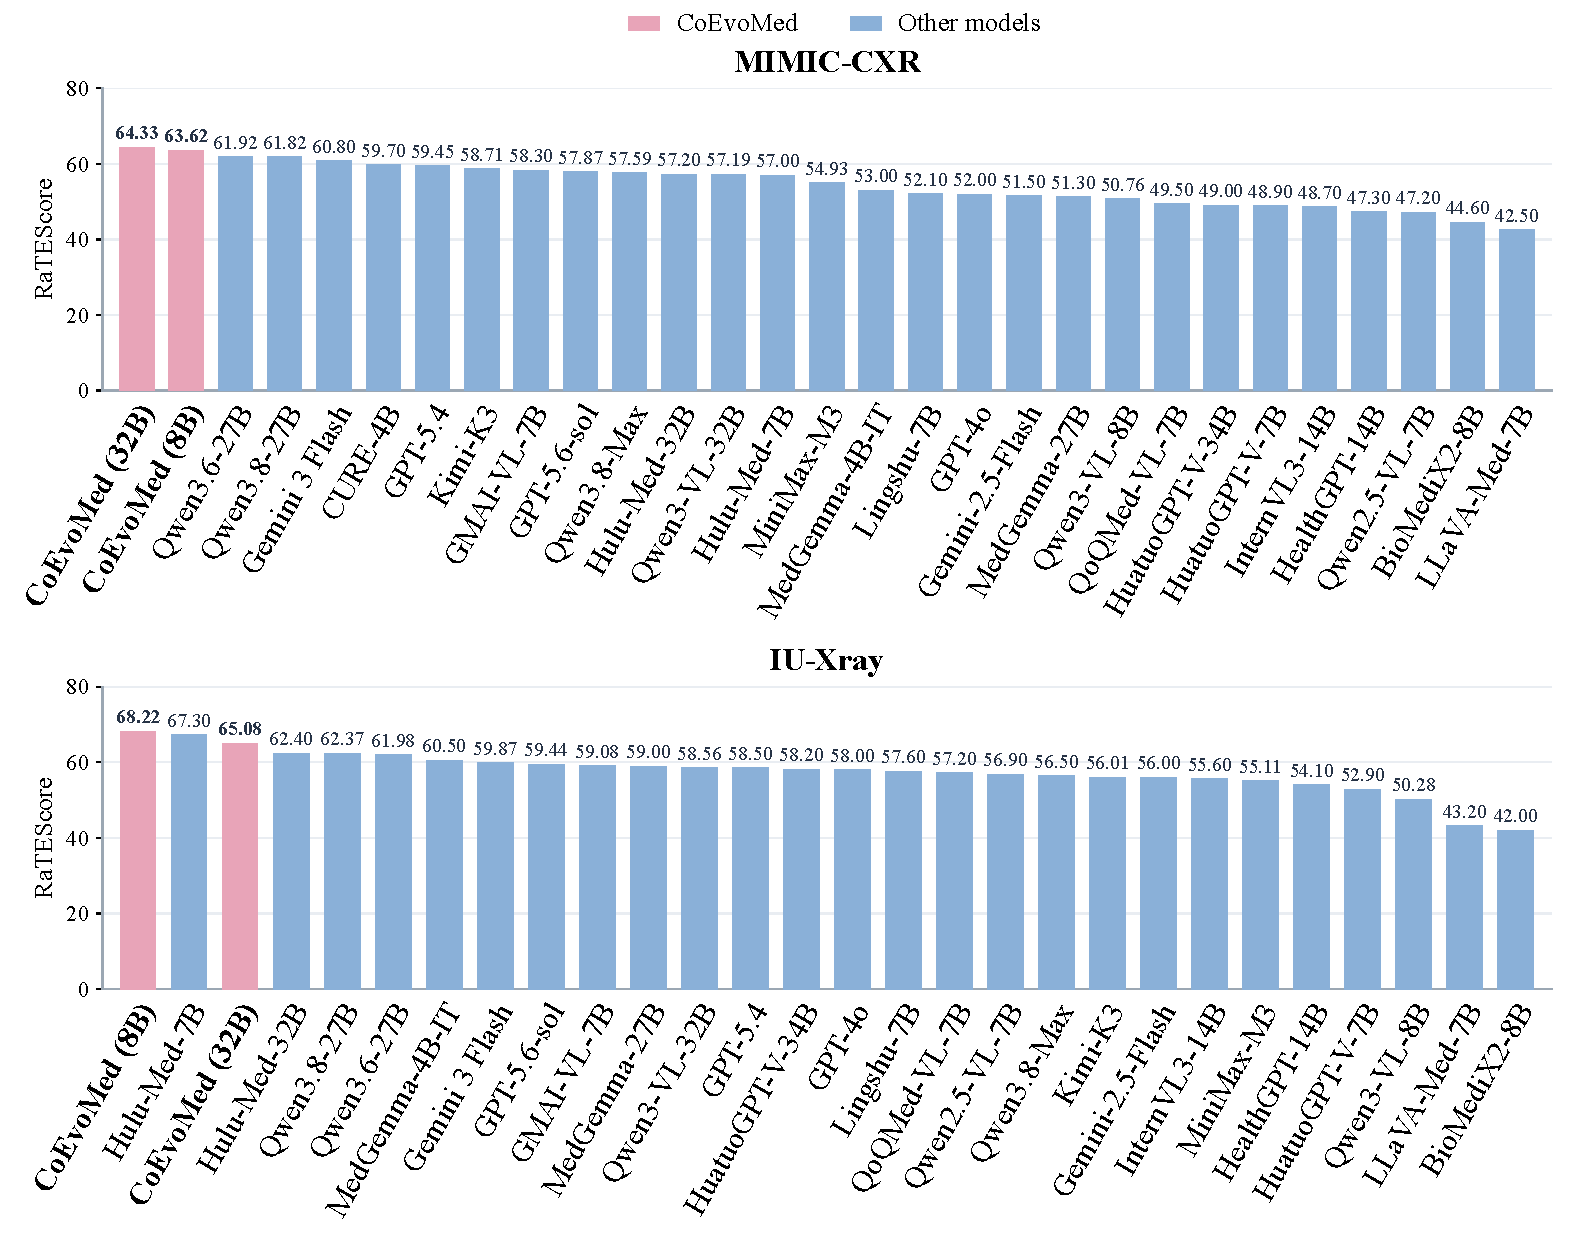
\includegraphics[width=0.90\linewidth,trim=0 14.8bp 0 4bp,clip]{figures/report_ratescore.pdf}
\caption{MIMIC-CXR（上，29个模型）与 IU-Xray（下，28个模型）的报告生成表现，分别按 RaTEScore（$\times100$）降序排列。粉色为 CoEvoMed，蓝色为基线。CURE-4B 采用 AGRG-29 + GRG 配置。补充指标见图~\ref{fig:report_lexical}。}
\label{fig:report_results}
\end{figure}

\paragraph{三维医学数据适用性。}
CoEvoMed 在图~\ref{fig:3d_main}的三项基准汇总比较中均位列首位，分别对应 M3D-VQA 宏平均准确率、3D-RAD 宏平均 ROUGE-1 与 AMOS-MM RaTEScore，将评价范围拓展至三维问答与报告生成。类别级结果、补充指标与评价协议见附录~\ref{app:3d}。

\begin{figure}[!htb]
\centering
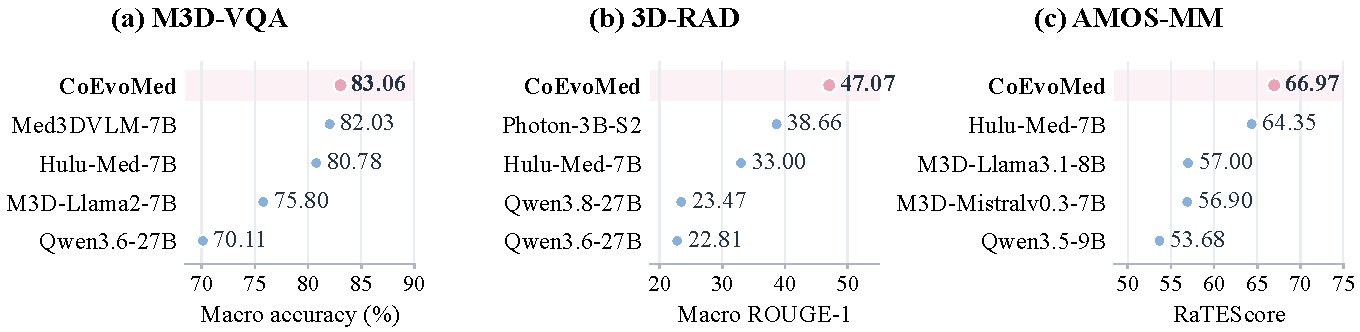
\includegraphics[width=\linewidth]{figures/three_d_main.pdf}
\caption{三维评测：（a）M3D-VQA 宏平均准确率；（b）3D-RAD 宏平均 ROUGE-1；（c）AMOS-MM RaTEScore，分数均乘以100。各面板展示 CoEvoMed（粉色），以及附录~\ref{app:3d}比较范围内按对应指标排名最高的四个基线（蓝色）。}
\label{fig:3d_main}
\end{figure}

\subsection{学习动态与机制分析}
\label{sec:analysis}
\label{sec:mechanisms}

我们考察学习轨迹、反馈与学习者状态的匹配性，以及构造原则效用的阶段依赖性。机制比较采用 VQA-RAD 与 MIMIC-CXR，完整结果与协议见附录~\ref{app:mechanisms}。

\paragraph{反馈与学习者状态的匹配性。}
各组从同一 R5 检查点出发，将数值能力统计与错误语义摘要共同替换为 R2、R3 或当前 R5 的验证反馈，指导课程分配与监督构造。当前反馈使 VQA-RAD 与 MIMIC-CXR 分别提高 2.62 个百分点与 2.77 分，均优于历史反馈（表~\ref{tab:ablations}，面板 A），支持课程适配与学习者当前能力状态及错误模式保持一致。

\paragraph{训练阶段依赖性。}
将原始与演化原则交叉应用于第2、5轮训练后的检查点（R2、R5），可观察到阶段依赖的监督效用（表~\ref{tab:ablations}，面板 B）。VQA-RAD 上，原始原则在 R2 领先 4.22 分，演化原则则在 R5 领先 8.26 分；MIMIC-CXR 上，演化原则的优势由 0.12 分扩大至 9.21 分。这种阶段依赖支持监督随学习者发展而修订，六项基准结果见附录~\ref{app:stage_transfer}。

\begin{table}[!htb]
\centering\small
\caption{机制消融：（A）R5 学习者的历史与当前反馈；（B）R2、R5 的原始与演化原则。VQA-RAD 为准确率（\%），MIMIC-CXR 为 RaTEScore（$\times100$）；参照为继续训练前分数。}
\label{tab:ablations}
\setlength{\tabcolsep}{3.5pt}
\renewcommand{\arraystretch}{1.08}
\begin{minipage}[t]{0.47\linewidth}
\vspace{0pt}
\begin{tabularx}{\linewidth}{Yrr}
\toprule
\multicolumn{3}{l}{\textbf{A. R5 学习者的反馈来源}}\\
\midrule
设置 & VQA-RAD & MIMIC-CXR\\
\midrule
R5：训练前 & 73.61 & 59.00\\
R2 反馈 & 72.51 & 59.11\\
R3 反馈 & 71.84 & 58.16\\
\rowcolor{mainOurs} \textbf{R5 反馈} & 76.23 & 61.77\\
\bottomrule
\end{tabularx}
\end{minipage}\hfill
\begin{minipage}[t]{0.50\linewidth}
\vspace{0pt}
\begin{tabularx}{\linewidth}{Yrr}
\toprule
\multicolumn{3}{l}{\textbf{B. 对训练阶段的依赖}}\\
\midrule
设置 & VQA-RAD & MIMIC-CXR\\
\midrule
R2：训练前 & 61.64 & 53.31\\
R2：原始原则 & 63.42 & 56.35\\
R2：演化原则 & 59.20 & 56.47\\
\midrule
R5：训练前 & 73.61 & 59.00\\
R5：原始原则 & 67.97 & 52.56\\
\rowcolor{mainOurs} \textbf{R5：演化原则} & 76.23 & 61.77\\
\bottomrule
\end{tabularx}
\end{minipage}
\end{table}

\paragraph{跨骨干适用性。}

Gemma-3-4B-IT 在 R7 达到 70.73\% 的 VQA 语义准确率与 65.89 的 MIMIC-CXR RaTEScore，较 Base 分别提高 22.39 和 16.23 分（图~\ref{fig:gemma_trajectory}）。同一检查点同时取得观测范围内并列最高的 VQA 准确率与最高报告分数，支持框架在更小规模、Qwen 家族之外的适用性。

\begin{figure}[!htb]
\centering
\vspace{-6pt}
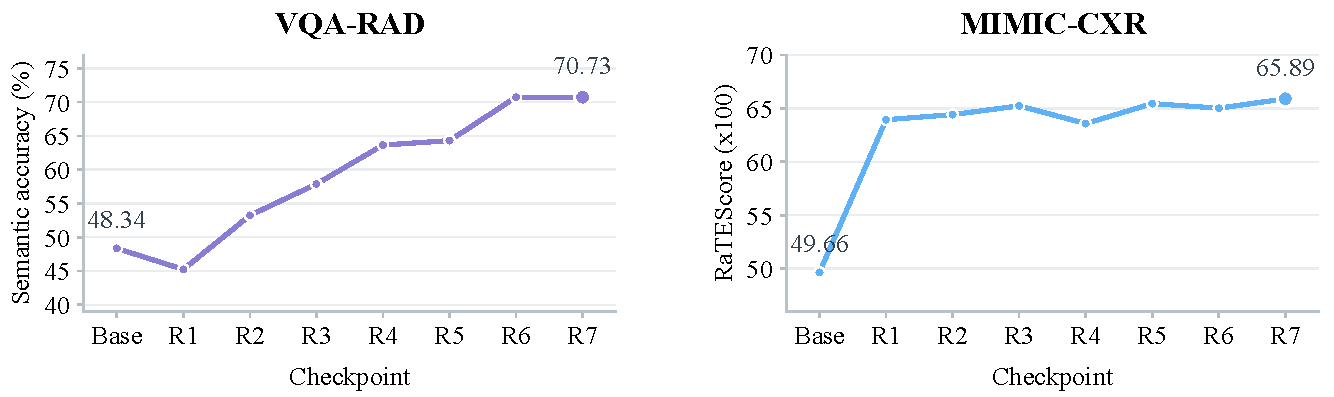
\includegraphics[width=0.85\linewidth]{figures/gemma_trajectory.pdf}
\caption{Gemma-3-4B-IT 从 Base 到 R7 的跨骨干验证。VQA-RAD 使用语义准确率（\%），MIMIC-CXR 使用乘以 100 的 RaTEScore。R7 的两项成绩来自同一 checkpoint。}
\label{fig:gemma_trajectory}
\end{figure}
\vspace{-10pt}
\begin{figure}[H]
\noindent\begin{minipage}[t]{0.40\textwidth}
\vspace{0pt}
\textbf{学习轨迹。} 图~\ref{fig:task_qa}显示，R1--R6 中属性问答提升、器官识别趋稳，定位问答在回落后恢复。这些分化的轨迹表明，不同任务的能力发展并不同步，为构造原则修订与构造分配提供状态信息。图~\ref{fig:trajectory}显示 SLAKE、PathVQA 与 IU-Xray 整体提升，并在 R7--R8 达到观测峰值。两组结果将学习者响应与外部基准性能联系起来，分别刻画能力发展及其在独立外部基准上的表现。
\end{minipage}\hfill
\begin{minipage}[t]{0.56\textwidth}
\vspace{0pt}\centering
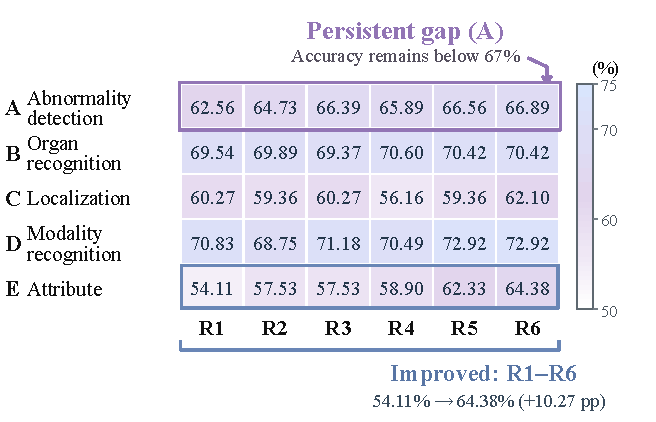
\includegraphics[width=\linewidth]{figures/task_qa_heatmap.pdf}
\caption{Qwen3-VL-8B 学习者在完成 R1--R6 训练后，于验证集上五类选定问答任务的准确率（\%）。}
\label{fig:task_qa}
\end{minipage}
\end{figure}
\vspace{-10pt}
\begin{figure}[H]
\centering
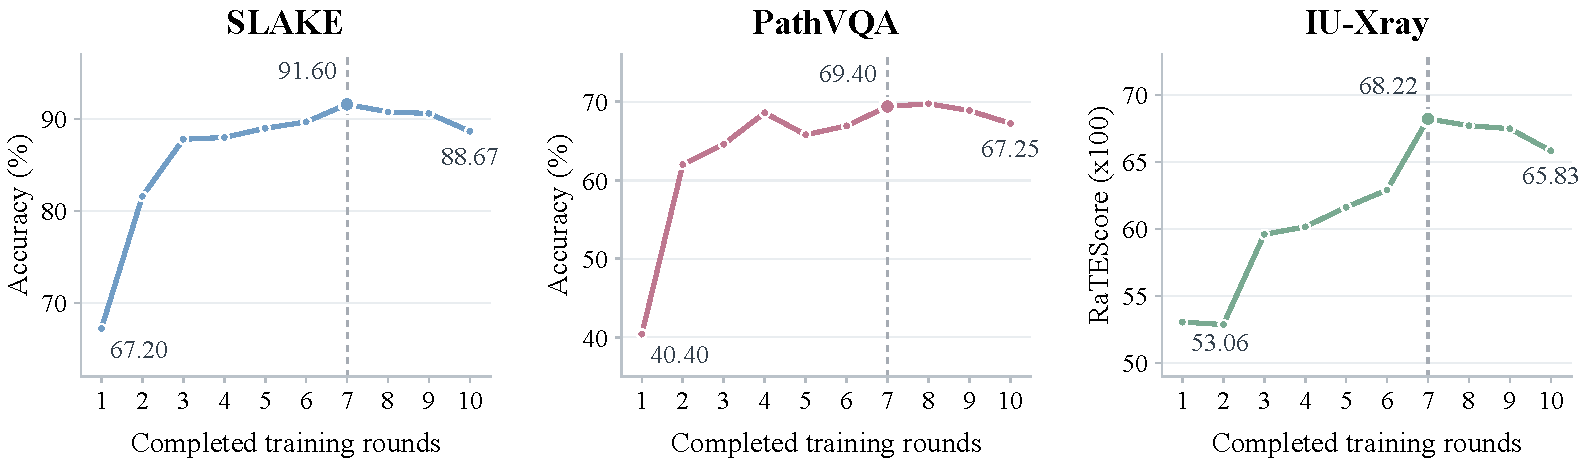
\includegraphics[width=0.85\linewidth]{figures/evolution_trajectory.pdf}
\caption{CoEvoMed-8B 的学习轨迹。虚线标记六项二维主结果统一采用的 R7 检查点。}
\label{fig:trajectory}
\end{figure}
\vspace{-12pt}
\FloatBarrier
\section{结论}
\label{sec:conclusion}

CoEvoMed 将监督构造视为医学视觉语言学习中持续演化的组成部分。构造原则随学习者的任务能力变化而修订，由此形成的监督进一步塑造后续能力发展。课程分配依据观测到的学习进展配置固定构造预算，与原则演化相互配合。多智能体协作将这两类适应过程结合起来，以医学证据为基础，使监督内容及其分配共同随学习者发展而调整。

二维视觉问答、报告生成、三维任务及不同骨干模型上的实验支持了该框架的有效性。不同反馈来源与训练阶段的比较进一步表明，使监督构造与学习者当前能力状态相匹配能够提高其效用。这些发现表明，监督构造方式与构造投入分配的协同调整，有助于提升医学多模态学习的效果。

\label{maintext:end}
\clearpage
\subsection*{AI 使用声明}
我们使用 AI 工具辅助论文写作与语言润色。我们已审阅相关文本，并对论文最终内容负责。

\subsection*{伦理声明}
本研究围绕医学多模态学习方法展开，仅使用既有公开或授权数据，未新增患者招募或开展临床干预。相关风险包括缺乏证据支持的医学陈述、标注错误传播，以及源数据或模型偏差的放大。CoEvoMed 通过证据约束的监督构造与验证处理合成监督中的事实不一致问题。源数据的访问与衍生产物的再分发受原数据集的许可、访问条件及隐私要求约束。临床应用需要独立验证、跨患者群体评估及专业临床监督。

\subsection*{可复现性声明}
第~\ref{sec:problem}--\ref{sec:method}节给出问题建模与核心机制，附录~\ref{app:algorithm}提供训练伪代码。附录~\ref{app:implementation}记录学习者训练设置、课程规划器初始化、PPO 超参数、监督预算与任务构成、原则接受准则、智能体模型及硬件配置。附录~\ref{app:evaluation}统一说明二维与三维评测划分及输入、数据来源与链接、证据加工、任务验证集构建、评价指标、检查点选择及反馈与外部评价的独立性。附录~\ref{app:mechanisms}给出消融设置与完整结果，附录~\ref{app:formalization}给出形式化定义与累积增益推导。

\bibliography{iclr2027_conference}
\bibliographystyle{iclr2027_conference}
\appendix
\clearpage
\section{完整训练过程}
\label{app:algorithm}

算法~\ref{alg:coevomed}概括共演化闭环。其中 $\pi_\theta$ 为 Actor 的 softmax 分布，$\mu$ 为加入均匀探索后的实际执行策略。附录~\ref{app:implementation}给出预算、训练混合、PPO 设置与原则修订规则。

\begin{algorithm}[H]
\small
\setlength{\tabcolsep}{4pt}
\renewcommand{\arraystretch}{1.08}
\begin{tabularx}{\linewidth}{@{}rY@{}}
\toprule
\multicolumn{2}{@{}p{\linewidth}@{}}{\textbf{输入：}学习者 $M_0$、原则集 $\Sigma_0$、已初始化的课程 Actor--Critic、验证集 $\mathcal V$、支持证据集 $\mathcal S$ 与时域 $E$。}\\
\multicolumn{2}{@{}p{\linewidth}@{}}{\textbf{输出：}学习者检查点序列 $\mathcal K_E=(M_0,\ldots,M_E)$ 与最终原则集 $\Sigma_E$。}\\
\midrule
1 & 在 $\mathcal V$ 上评估 $M_0$ 得到 $o_0$；初始化 $h_0=(o_0)$、$\mathcal K_0=(M_0)$ 与使用量统计。\\
2 & \textbf{for} $e=0,\ldots,E-1$ \textbf{do}\\
3 & \hangindent=1em\hangafter=1\quad $\mathbf{s}_e\leftarrow\Phi(h_e)$; $\mu_{\mathrm{old}}\leftarrow0.8\pi_\theta(\cdot\mid\mathbf{s}_e)+0.05$.\\
4 & \hangindent=1em\hangafter=1\quad $a_e\sim\operatorname{Categorical}(\mu_{\mathrm{old}})$; $\ell_e^{\mathrm{old}}\leftarrow\log\mu_{\mathrm{old}}(a_e)$.\\
5 & \hangindent=1em\hangafter=1\quad $\boldsymbol q_e\leftarrow\mathcal A(a_e,h_e)$，保持任务配额（式~\ref{eq:quota}）。\\
6 & \hangindent=1em\hangafter=1\quad 按 $\boldsymbol q_e$ 规划修复与保持目标，并从 $\mathcal S$ 选取支持事实。\\
7 & \hangindent=1em\hangafter=1\quad 依据 $\Sigma_e$ 构造并验证 $\mathcal D_e^{\mathrm{syn}}$；记录来源与原则版本。\\
8 & \hangindent=1em\hangafter=1\quad $\mathcal D_e^{\mathrm{mix}}\leftarrow\operatorname{Mix}(\mathcal D_e^{\mathrm{syn}},\mathcal R_e)$; $M_{e+1}\leftarrow\mathcal U(M_e,\mathcal D_e^{\mathrm{mix}})$.\\
9 & \hangindent=1em\hangafter=1\quad 在相同的 $\mathcal V$ 上评估 $M_{e+1}$，得到 $o_{e+1}$ 与成对学习响应。\\
10 & \hangindent=1em\hangafter=1\quad $r_e\leftarrow G_e$（式~\ref{eq:gain}）；$\mathcal K_{e+1}\leftarrow(\mathcal K_e,M_{e+1})$。\\
11 & \hangindent=1em\hangafter=1\quad $h_{e+1}\leftarrow(h_e,a_e,r_e,o_{e+1})$; $\mathbf{s}_{e+1}\leftarrow\Phi(h_{e+1})$.\\
12 & \hangindent=1em\hangafter=1\quad 依据 $(\mathbf{s}_e,a_e,r_e,\mathbf{s}_{e+1})$ 计算单步优势估计与价值目标。\\
13 & \hangindent=1em\hangafter=1\quad \textbf{for} $k=1,\ldots,4$ \textbf{do}\\
14 & \hangindent=2em\hangafter=1\qquad $\mu_{\mathrm{new}}\leftarrow0.8\pi_\theta(\cdot\mid\mathbf{s}_e)+0.05$; $\rho_e\leftarrow\exp\!\left(\log\mu_{\mathrm{new}}(a_e)-\ell_e^{\mathrm{old}}\right)$.\\
15 & \hangindent=2em\hangafter=1\qquad 使用裁剪 PPO（$\rho_e$）、价值损失与熵项 $H(\mu_{\mathrm{new}})$ 更新 Actor--Critic。\\
16 & \hangindent=1em\hangafter=1\quad \textbf{end for}\\
17 & \hangindent=1em\hangafter=1\quad 按原则版本更新窗口统计；$\Sigma_{e+1}\leftarrow\Sigma_e$。\\
18 & \hangindent=1em\hangafter=1\quad \textbf{if} 演化窗口结束 \textbf{then}\\
19 & \hangindent=2em\hangafter=1\qquad 依据残余错误提出符合修订条件的原则候选，保持目标能力与医学事实不变。\\
20 & \hangindent=2em\hangafter=1\qquad 在相同配额下，依据当前与候选原则，使用 $N=100$ 个相同证据任务构造并验证配对样本，得到可用索引集 $I_{\mathrm{cur}},I_{\mathrm{cand}}$。\\
21 & \hangindent=2em\hangafter=1\qquad $\Delta_{\mathrm{use}}\leftarrow\dfrac{|I_{\mathrm{cand}}|-|I_{\mathrm{cur}}|}{N}$; $\rho_{\mathrm{pair}}\leftarrow\dfrac{|I_{\mathrm{cand}}\cap I_{\mathrm{cur}}|}{N}$.\\
22 & \hangindent=2em\hangafter=1\qquad 若 $\rho_{\mathrm{pair}}\geq0.60$，由原则修订智能体对至多30组共同可用的配对样本进行语义审查。\\
23 & \hangindent=2em\hangafter=1\qquad 当 $|I_{\mathrm{cand}}|/N\geq0.80$、$\Delta_{\mathrm{use}}\geq-0.05$、$\rho_{\mathrm{pair}}\geq0.60$ 且语义审查通过时，替换 $\Sigma_{e+1}$ 中对应原则。\\
24 & \hangindent=1em\hangafter=1\quad \textbf{end if}\\
25 & \textbf{end for}\\
26 & \textbf{return} $\mathcal K_E,\Sigma_E$.\\
\bottomrule
\end{tabularx}
\caption{CoEvoMed：学习响应驱动的监督构造。}
\label{alg:coevomed}
\end{algorithm}

符合修订条件的原则在演化窗口内具有充分使用量且净修复不为正。语义审查要求修订实际体现在生成样本中、改善与目标错误的契合度，并保持证据支持。接受的修订于下一轮生效；拒绝或暂缓的候选均保留当前版本。保存的 $\ell_e^{\mathrm{old}}$ 在四个 PPO 优化 epoch 中保持不变。

构造阶段使用选定事实而不直接读取图像，验证阶段结合图像检查候选样本。将监督样本与生成它们所用的构造原则版本关联，可把原则使用量与对应能力的验证变化相联系。训练混合排除 $\mathcal V$ 与外部基准 $\mathcal B_{\mathrm{ext}}$。保存的模型序列用于离线轨迹分析；六项二维 8B 主结果统一采用 R7（附录~\ref{app:checkpoint_selection}）。外部基准结果不返回适应闭环。


\section{训练设置}
\label{app:implementation}

\paragraph{学习者训练。}
主要学习者为 Qwen3-VL-8B-Instruct，Qwen3-VL-32B 用于二维任务的规模扩展实验。各轮训练均从上一轮学习者参数继续更新，训练数据由已接受的证据约束监督 $\mathcal D_e^{\mathrm{syn}}$ 与规定的原始或回放数据 $\mathcal R_e$ 混合构成。监督微调（FullSFT）更新语言模型与多模态 merger 的全部参数，同时冻结视觉塔。二维训练配置规定每轮完整遍历 $\mathcal D_e^{\mathrm{mix}}$ 一次，训练时长由 epoch 数决定（\texttt{max\_steps=-1}）。采用 AdamW~\citep{loshchilov2019decoupled}，参数为 $\beta_1=0.9$、$\beta_2=0.999$、$\epsilon=10^{-8}$，权重衰减为 $0.1$，bias 等免衰减参数除外。语言模型与 merger 的学习率均为 $10^{-5}$，采用余弦衰减，预热比例为 $0.03$。训练使用3个节点，每节点8张 NVIDIA A100 80\,GB，共24张 GPU；单卡 batch size 为1，梯度累积为1步，全局有效 batch size 为24。计算采用 BF16 与 DeepSpeed ZeRO-3~\citep{rajbhandari2020zero}，并关闭梯度检查点。对于体数据输入，开启 TF32，并将每个切片帧的像素数量限制为65,536--196,608。
\paragraph{智能体分工与模型。}
五个智能体共同完成监督构造、课程分配与原则修订。证据选择智能体使用 deepseek-v4-flash 选择支持证据，监督构造智能体使用同一模型依据构造原则生成训练样本。证据核验智能体使用 Qwen3.6-27B 评估证据支持与事实一致性。课程规划器根据能力反馈与学习进展分配构造投入：学习得到的 Actor--Critic 选择分配动作，deepseek-v4-flash 明确构造目标，并为监督初始化提供动作标签。原则修订智能体使用 deepseek-v4-flash 根据学习响应提出并评估构造原则修订。Qwen3.6-27B 还用于事实证据抽取与验证集标注。

\paragraph{每轮监督规模与任务构成。}
每轮训练引入50,000条通过证据验证的监督样本，组成$\mathcal D_e^{\mathrm{syn}}$，视觉问答（VQA）与报告生成（caption）的样本数量比约为 $7:3$。在 VQA 子集中，多项选择题、二值判断题与简短回答题的样本数量比约为 $92:4:4$。上述两级比例分别描述任务族之间的监督构成及问答任务内部的回答形式分布。

\paragraph{学习者训练目标。}
\label{app:learner_objective}
对于可训练参数为 $\phi$ 的学习者，式~\ref{eq:learning_dynamics}的更新最小化
\begin{equation}
\mathcal L_e(\phi)=-\E_{(v,x,y)\sim\mathcal D_e^{\mathrm{mix}}}
\sum_{j=1}^{|y|}\log p_\phi(y_j\mid v,x,y_{<j}),
\label{eq:student}
\end{equation}
其中 $v$、$x$、$y$ 分别表示视觉输入、指令与目标回答。每次更新后，在固定任务验证样本上测量学习响应。

\paragraph{课程规划器初始化。}
课程规划器将40维状态映射至隐层宽度为128与64的共享两层 MLP，并连接四动作 Actor 与标量 Critic。四类课程动作分别为均衡、修复优先、弱点聚焦与保持优先。依据基线评测统计构造800条能力状态，覆盖均衡表现、整体薄弱、局部薄弱与能力回退四类情形，由教师模型 deepseek-v4-flash 标注课程动作。按状态组划分640条训练状态与160条验证状态，通过交叉熵监督初始化共享 MLP 与 Actor，并选取验证表现最佳的第5个 epoch 检查点。Critic 输出头的权重与偏置初始化为零，随后依据真实反馈学习。上述800条状态用于监督初始化，与在线学习者交互分别计数。

\paragraph{PPO 优化。}
每个课程轮次包含决策、监督构造、学习者训练与验证反馈，形成一条环境转移。Actor--Critic 在每轮结束后更新一次，对该轮交互记录执行四个优化 epoch。单步交互记录下，广义优势估计简化为单步时序差分估计。采用 Adam~\citep{kingma2015adam}，学习率为 $3\times10^{-4}$，折扣因子 $\gamma=0.90$，GAE 参数 $\lambda=0.95$，裁剪阈值为0.20，价值损失与熵正则系数分别为0.50与0.01，梯度范数上限为0.50。PPO 更新课程规划器，外部大语言模型的权重保持固定。到达原则演化边界时，先优化规划器，再修订构造原则。

\paragraph{混合策略下的采样与概率比。}
令 $\pi_\theta(\cdot\mid s)=\operatorname{softmax}(\operatorname{Actor}_\theta(s))$。实际执行策略将 Actor 分布与四动作上的均匀探索混合：
\[
\mu_\theta(a\mid s)=0.8\pi_\theta(a\mid s)+0.05.
\]
动作从 $\mu_{\theta_{\mathrm{old}}}$ 采样，并在采样时保存对数概率 $\ell_e^{\mathrm{old}}=\log\mu_{\theta_{\mathrm{old}}}(a_e\mid \mathbf{s}_e)$；该值在四个优化 epoch 中保持固定。每个 epoch 在已保存的状态与动作上重新计算混合策略概率，得到 PPO 概率比
\[
\rho_e(\theta)=\exp\!\left(\log\mu_\theta(a_e\mid \mathbf{s}_e)-\ell_e^{\mathrm{old}}\right)
=\frac{\mu_\theta(a_e\mid \mathbf{s}_e)}{\mu_{\theta_{\mathrm{old}}}(a_e\mid \mathbf{s}_e)}.
\]
熵正则同样作用于 $\mu_\theta$。该执行策略对应式~\ref{eq:objective}中的分配策略。

\paragraph{基于学习进展的奖励。}
奖励来自真实学习者更新后的验证增益。VQA 采用准确率，报告生成采用 $0.5\,\mathrm{ROUGE\mbox{-}L}+0.3\,\mathrm{BLEU\mbox{-}4}+0.2\,\mathrm{METEOR}$。各任务增益先在任务族内平均，再对 VQA 与报告两族等权汇总，与式~\ref{eq:gain}一致。

\paragraph{原则修订与选择。}
持续保留的监督构造原则规定问题意图、证据与回答的关联、概念对比及多样性。各窗口内观测到的学习响应识别使用量充分且净修复不为正的原则，修订智能体根据残余错误摘要提出候选，同时保持目标能力与医学事实不变。当前原则与候选原则在相同的 $N>0$ 组支持证据分配上比较。以 $I_{\mathrm{cur}}$ 与 $I_{\mathrm{cand}}$ 表示产出可用监督的分配索引集合，相对可用产出率与配对覆盖率为
\begin{equation}
\Delta_{\mathrm{use}}=\frac{|I_{\mathrm{cand}}|-|I_{\mathrm{cur}}|}{N},
\qquad
\rho_{\mathrm{pair}}=\frac{|I_{\mathrm{cand}}\cap I_{\mathrm{cur}}|}{N}.
\label{eq:strategy_comparison}
\end{equation}
比较采用 $N=100$ 个匹配任务，分母包含全部请求任务。接受候选须满足
\[
\frac{|I_{\mathrm{cand}}|}{N}\geq0.80,\qquad
\Delta_{\mathrm{use}}\geq-0.05,\qquad
\rho_{\mathrm{pair}}\geq0.60,
\]
并通过明确的语义审查。配对覆盖达到门槛后，原则修订智能体考察至多30组共同可用的配对样本，确认修订实际体现于监督内容，且在保持证据支持的同时改善对目标错误语义的覆盖。仅改变措辞或替换同义词不计为改善。

可用监督产出率下降超过五个百分点、当前版本达到0.80而候选低于该门槛，或出现语义退化时，拒绝候选。其余因任务不足、数值条件未满足或语义改善未获确认的情况暂缓决定。两种情形均保留当前原则，接受的修订用于后续构造。选择依据配对监督比较，学习者响应则在后续训练轮次中评价。

\section{实验设置与评价}
\label{app:evaluation}
\label{app:3d}

我们在二维与三维基准上评估训练后的 CoEvoMed-8B，其中每个体数据表示为包含64个切片帧的视频。

\subsection{评测数据与输入}
\label{app:datasets_2d}

\paragraph{二维基准。}

本研究在六个公开二维医学基准上进行评测，覆盖放射与病理问答、医学文献图像理解及胸片报告生成。CoEvoMed 与本研究评测的基线统一采用相同的评测集与评分协议，评测规模见表~\ref{tab:datasets_2d}：VQA 按问答条目计数，MRG 按报告生成实例计数。

\begin{table}[H]
\centering\small
\caption{本研究二维评测所用数据集。规模指实际评测条目数，不指完整源数据集规模或独立患者数。VQA：视觉问答；MRG：医学报告生成。}
\label{tab:datasets_2d}
\setlength{\tabcolsep}{4pt}
\renewcommand{\arraystretch}{1.10}
\begin{tabularx}{\linewidth}{@{}lcrY@{}}
\toprule
基准 & 任务 & 条目数 & 视觉证据与标注来源\\
\midrule
VQA-RAD & VQA & 451 & 放射影像及临床医生撰写的问答。\\
SLAKE & VQA & 1,061 & 放射影像，结合医生标注的语义信息与医学知识库。\\
PMC-VQA & VQA & 33,430 & 从开放获取生物医学文献中的多类图像及图注构造问答。\\
PathVQA & VQA & 6,761 & 来源于教材和数字图书馆的病理图像及相关问答。\\
MIMIC-CXR & MRG & 2,343 & 胸部放射影像及配套临床报告。\\
IU-Xray & MRG & 590 & 胸片检查及配套放射报告。\\
\bottomrule
\end{tabularx}
\end{table}

VQA-RAD、SLAKE 与 PathVQA 侧重放射或病理领域的理解，PMC-VQA 则覆盖异质医学图像 \citep{lau2018dataset,liu2021slake,he2020pathvqa,zhang2024pmc}。MIMIC-CXR 与 IU-Xray 考察模型将影像证据组织为报告的能力 \citep{johnson2019mimic,demnerfushman2016preparing}。VQA 采用准确率；报告生成采用 RaTEScore 评价临床语义一致性，并以 METEOR、BLEU-1/2/3/4 和 ROUGE-1/2/L 衡量互补的文本一致性。

表~\ref{tab:main}中的医学基线包括 MedGemma~\citep{sellergren2025medgemma}、GMAI-VL~\citep{li2026gmai}和 MedDr~\citep{he2024meddr}。图~\ref{fig:report_results}与图~\ref{fig:report_lexical}中的报告生成比较还包括 Qwen2.5-VL~\citep{bai2025qwen25}和 HealthGPT~\citep{lin2025healthgpt}。


\paragraph{三维基准。}
\label{app:datasets_3d}

三维评测共包含18,883个条目，覆盖 M3D-VQA 的四选一识别、3D-RAD 的开放式问答与 AMOS-MM 的报告生成三类互补任务~\citep{bai2024m3d,gai2025threedrad,ji2024amosmm}。评测采用本地 M3D-VQA 测试划分的全部闭合题、本地 3D-RAD 测试划分的全部开放题，以及 AMOS-MM 验证划分的全部400例。

\begin{table}[H]
\centering\small
\caption{本地三维评测集的组成。序列数按各基准的媒体路径去重，表示媒体文件数而非独立患者数。AMOS-MM 采用其验证划分进行评测。}
\label{tab:datasets_3d}
\setlength{\tabcolsep}{4pt}
\renewcommand{\arraystretch}{1.10}
\begin{tabularx}{\linewidth}{@{}llYrr@{}}
\toprule
基准 & 原始划分 & 评测任务 & 条目数 & 序列数\\
\midrule
M3D-VQA & Test & 四选一问答 & 13,791 & 2,000\\
3D-RAD & Test & 开放式问答 & 4,692 & 2,354\\
AMOS-MM & Validation & 报告生成 & 400 & 400\\
\bottomrule
\end{tabularx}
\end{table}

M3D-VQA 考察成像平面、增强期相、器官识别、异常识别及解剖定位。3D-RAD 覆盖解剖与病理观察，异常特征、位置、类型及诊断，以及直径、大小和厚度的定量描述。AMOS-MM 评估较长影像所见的生成，参考内容涉及胸部、腹部及盆腔结构；评分采用 \emph{findings} 字段，不拼接 impression。参考答案仅用于评分，不作为推理输入。

\paragraph{三维输入与预处理。}
通用输入表示沿体积深度方向均匀采样64张切片，较短序列允许重复采样。切片以512像素为目标最长边缩放，按空间顺序保存为 H.264 MP4（yuv420p、16像素对齐、1 fps）。原生三维模型保留各自的输入适配器；Photon S2~\citep{fang2026photon}的本地评测使用32张切片重构的体积。解码采用贪心策略。所选数据的条目 ID 无重复、参考答案非空，引用媒体均可用。预处理在采样前排除四个 M3D 源序列中的109个不可识别图像成员，保留全部关联问题。

\paragraph{三维指标与汇总方式。}
M3D-VQA 同时报告全部问题的总体准确率与五类任务的宏平均准确率。Plane、Phase、Organ 各包含2,000道题，Abnormality 与 Location 分别包含4,831和2,960道题。3D-RAD 的异常检测、图像观察与医学计算分别包含2,666、1,024和1,002道题。本次评测采用 WMT~13a 分词、无平滑的 corpus BLEU-1 及 ROUGE-1 F1，各任务分别对其四个、两个和三个子任务分数等权平均。AMOS-MM 采用 RaTEScore、BLEU-1、ROUGE-L 与 METEOR。所有分数统一乘以100。正文图~\ref{fig:3d_main}分别采用 M3D-VQA 的类别宏平均准确率、3D-RAD 三类任务 ROUGE-1 的均值，以及 AMOS-MM 的 RaTEScore。


\subsection{基准补充结果}
\label{app:report_lexical}

\paragraph{报告生成指标。}

图~\ref{fig:report_lexical}在相同的两个报告基准上补充 METEOR、BLEU-1/2/3/4 和 ROUGE-1/2/L，与正文的 RaTEScore 比较相互补充。这些指标刻画生成报告与参考报告的文本重合程度，图~\ref{fig:report_results}中的 RaTEScore 提供临床语义层面的评价。

\begin{figure}[!htb]
\centering
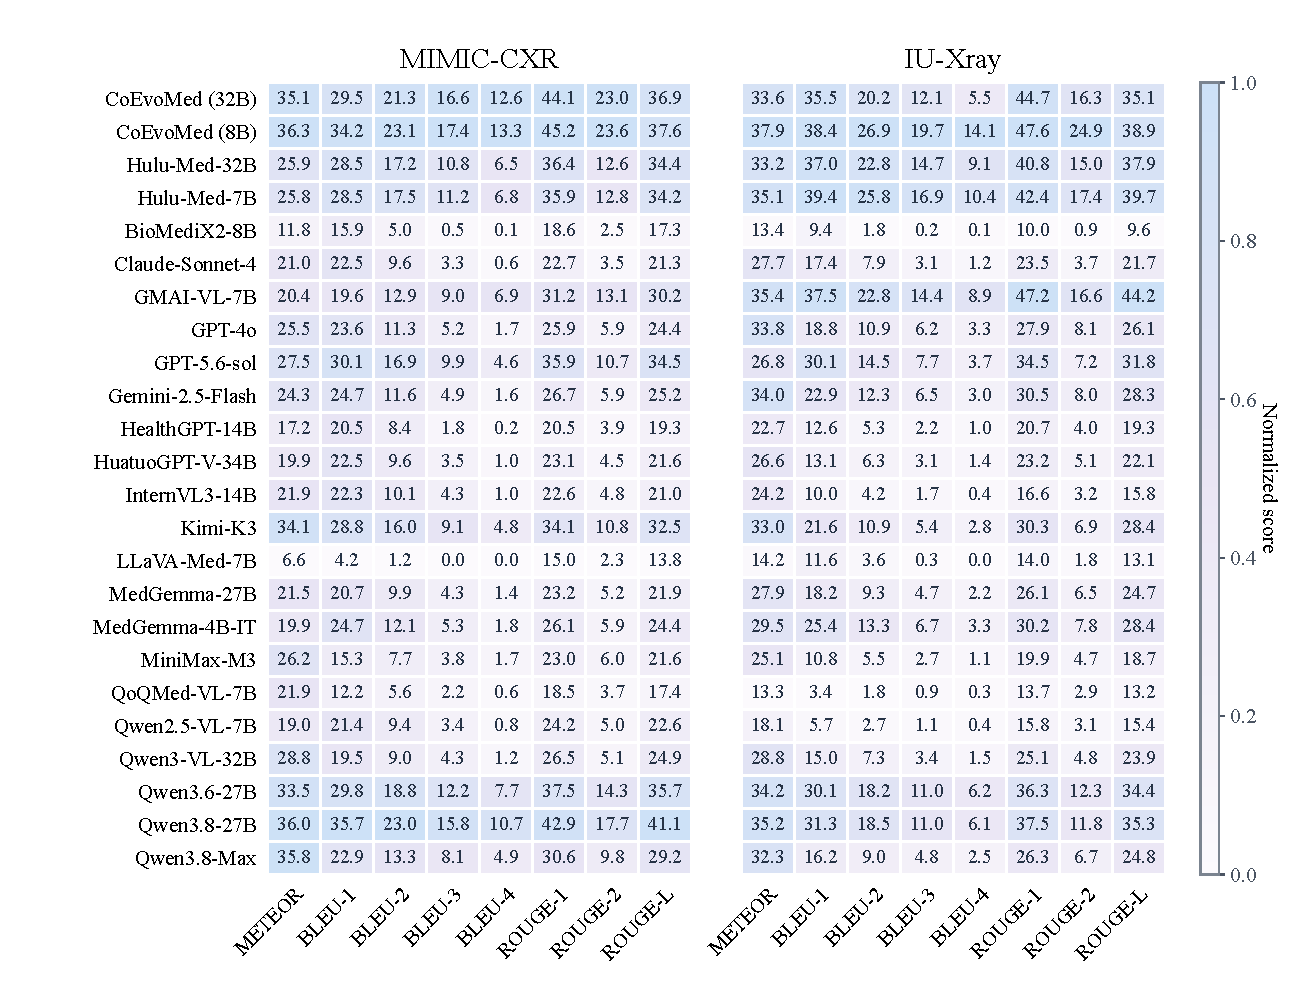
\includegraphics[width=\linewidth]{figures/report_lexical.pdf}
\caption{MIMIC-CXR 与 IU-Xray 报告生成的补充文本指标。单元格显示 0--100 标度的分数，保留一位小数；颜色在各数据集的每项指标内作最小--最大归一化，指标越高越好。``--''表示缺失值，不作为零分处理。}
\label{fig:report_lexical}
\end{figure}

\paragraph{三维基准结果。}

图~\ref{fig:3d_appendix_profiles}展示三维识别、开放问答与报告生成结果。CoEvoMed 在 M3D-VQA 五类任务中均取得最高准确率，总体准确率为80.11\%（11,048/13,791），类别宏平均为83.06\%；Med3DVLM-7B（Med3DVLM-Qwen-2.5-7B）~\citep{xin2025med3dvlm}的总体准确率为79.18\%。这些结果支持 CoEvoMed 在互补三维医学任务上的适用性。

\begin{figure}[!htbp]
\centering
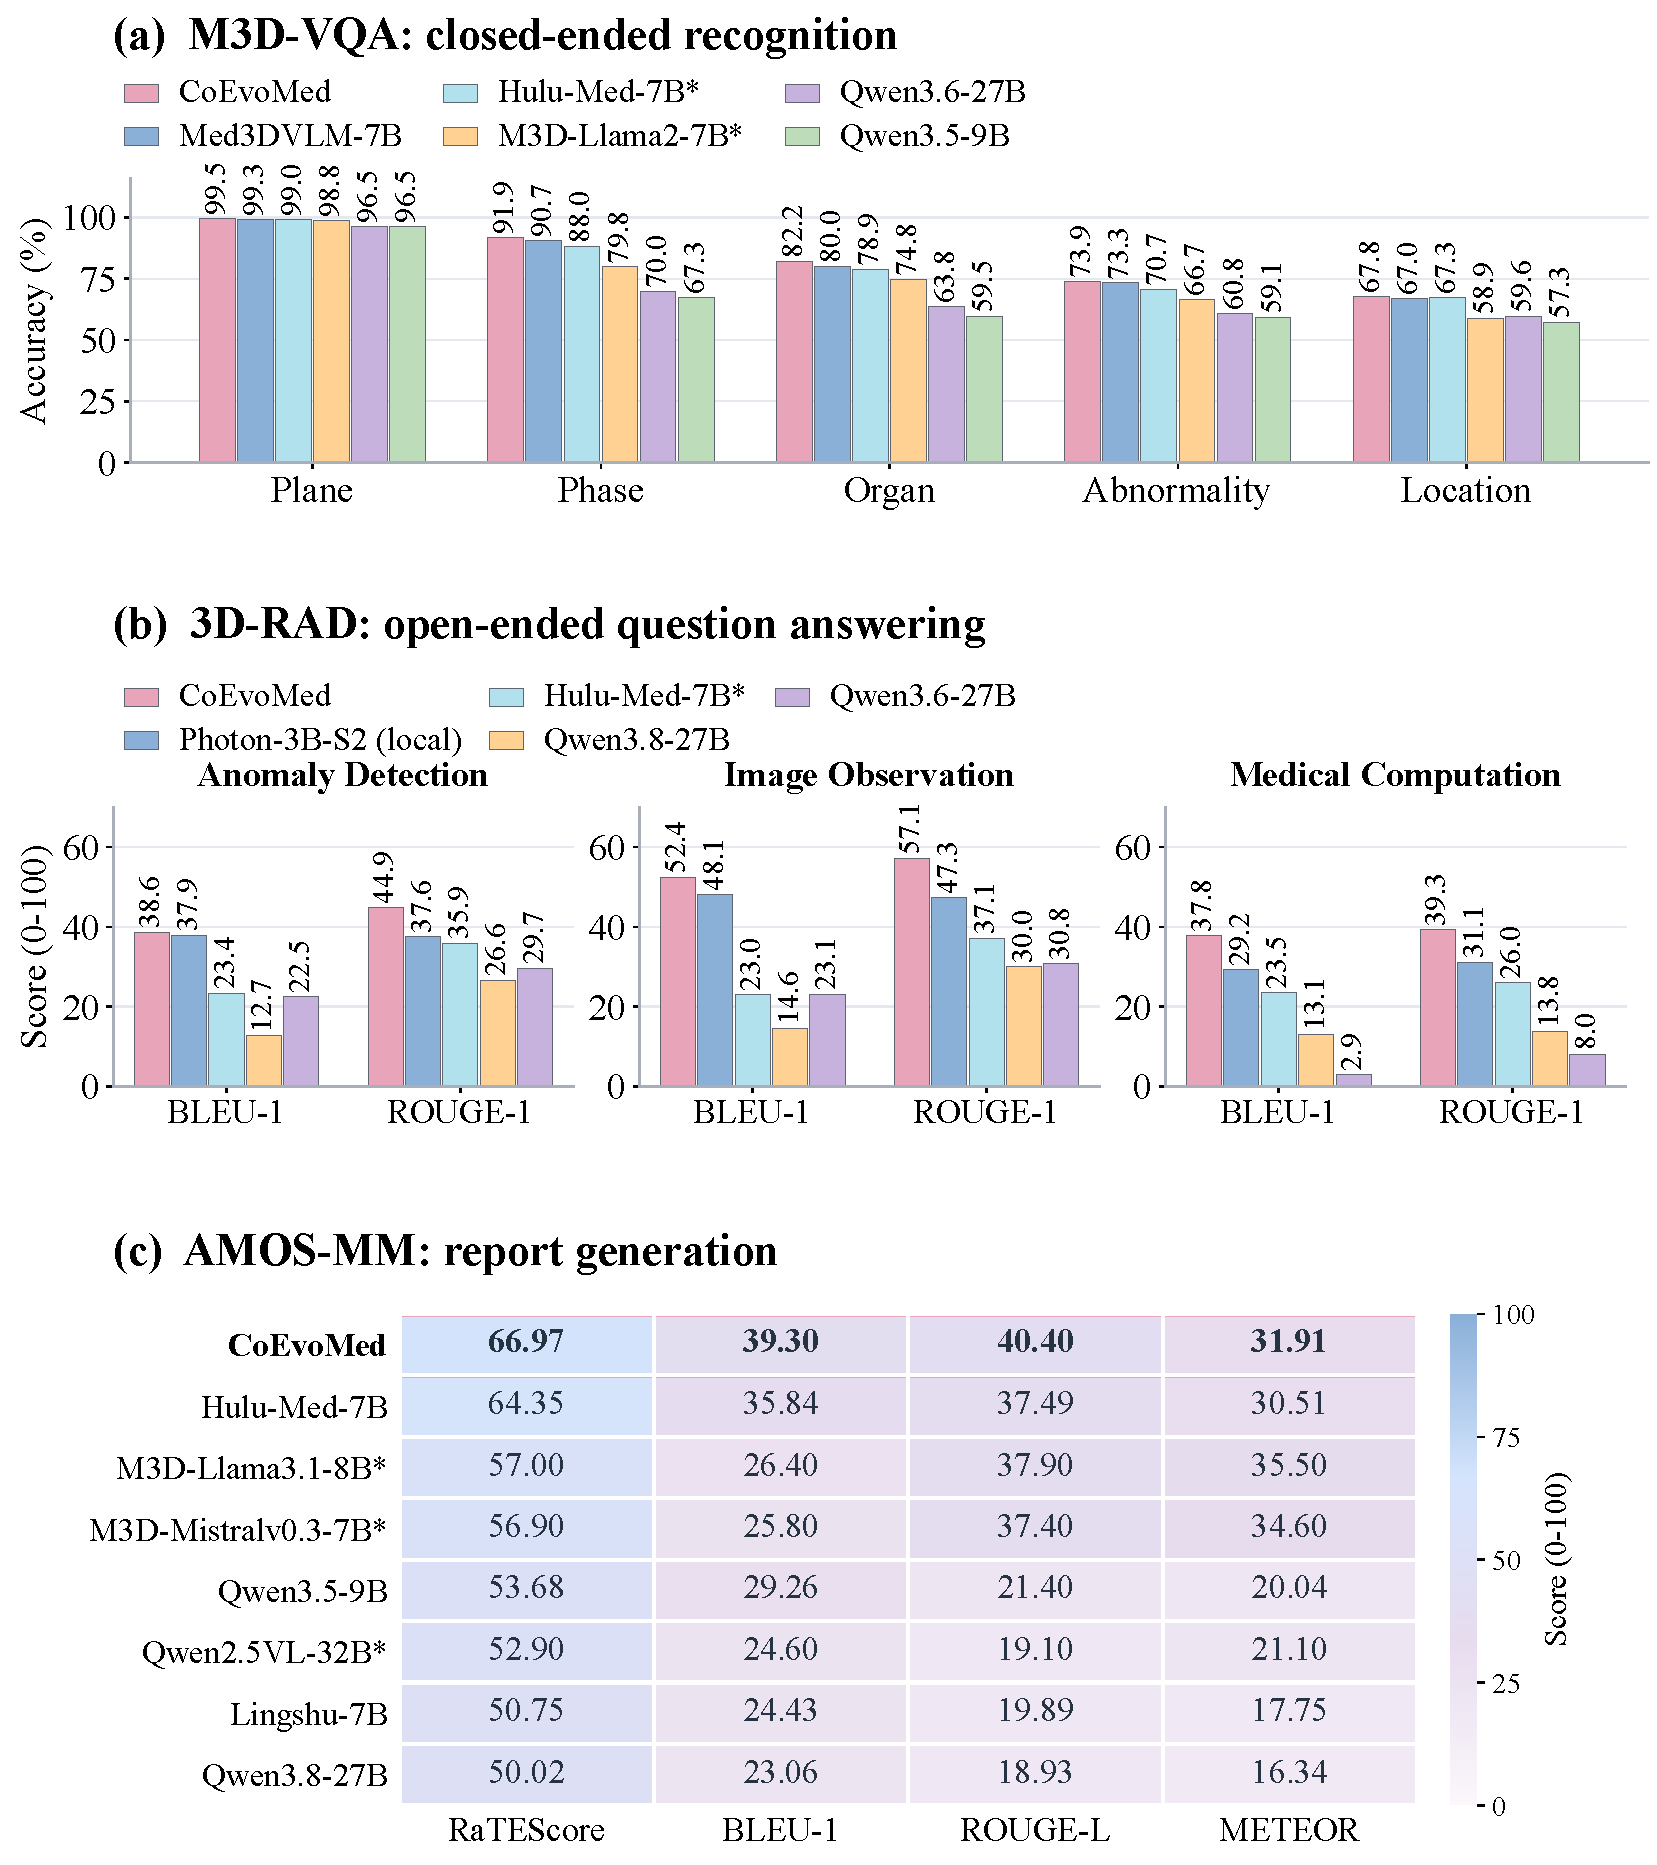
\includegraphics[width=0.84\linewidth]{figures/three_d_appendix_profiles.pdf}
\caption{三维基准细分结果。(a) M3D-VQA 五类闭合题的准确率。(b) 3D-RAD 三类开放任务的 BLEU-1 与 ROUGE-1；Photon 采用 S2 本地评测。(c) AMOS-MM 报告生成指标，标注原始数值并使用固定 0--100 色阶。各部分均展示 CoEvoMed 与排名靠前的可用基线：(a) 按类别平均准确率选取五个，(b) 按任务平均 ROUGE-1 选取四个，(c) 按 RaTEScore 选取七个。全部指标统一乘以100。星号标记 \citet{jiang2025hulumed} 的文献结果。}
\label{fig:3d_appendix_profiles}
\end{figure}


\subsection{支持证据与验证集的构建}

支持集 $\mathcal S$ 提供监督构造所需的源证据。按任务组织的验证集 $\mathcal V=\{\mathcal V_t\}_{t\in\mathcal T}$ 通过提供能力估计、错误语义与课程回报，评估学习者能力并指导适应过程。外部基准集合 $\mathcal B_{\mathrm{ext}}$ 用于报告最终模型及中间检查点的表现。下文介绍支持证据与验证集的构建。

任务划分 $\mathcal T$ 定义验证反馈所用的任务单元，下文列出支持集来源及其监督构造用途。二维与三维任务的评测数据及输入处理统一见附录~\ref{app:datasets_2d}。Gemma-3-4B-IT 的学习轨迹见正文图~\ref{fig:gemma_trajectory}，InternVL3-9B 的结果见附录~\ref{app:internvl}；InternVL3-9B 的两项任务分别训练独立模型。

\paragraph{二维支持集。}
\label{app:support_2d}
二维支持集包含来自11个数据集的259,767条源记录，覆盖医学论文图像、放射影像、病理图像及相关文本与标签。图~\ref{fig:support_composition}展示来源组成，表~\ref{tab:support_links}提供各数据集的官方资源链接。

\paragraph{三维支持集。}
\label{app:support_3d}
三维支持集包含来自5个数据集的215,657条源记录，其中包括209,329条问答与6,328条报告，覆盖解剖识别、定位、异常表征及报告生成。问答对应4,228个唯一视频，每个视频包含64帧有序切片。图~\ref{fig:support_composition}展示来源组成，表~\ref{tab:support_links}提供各数据集的官方资源链接。

\begin{figure}[!htb]
\centering
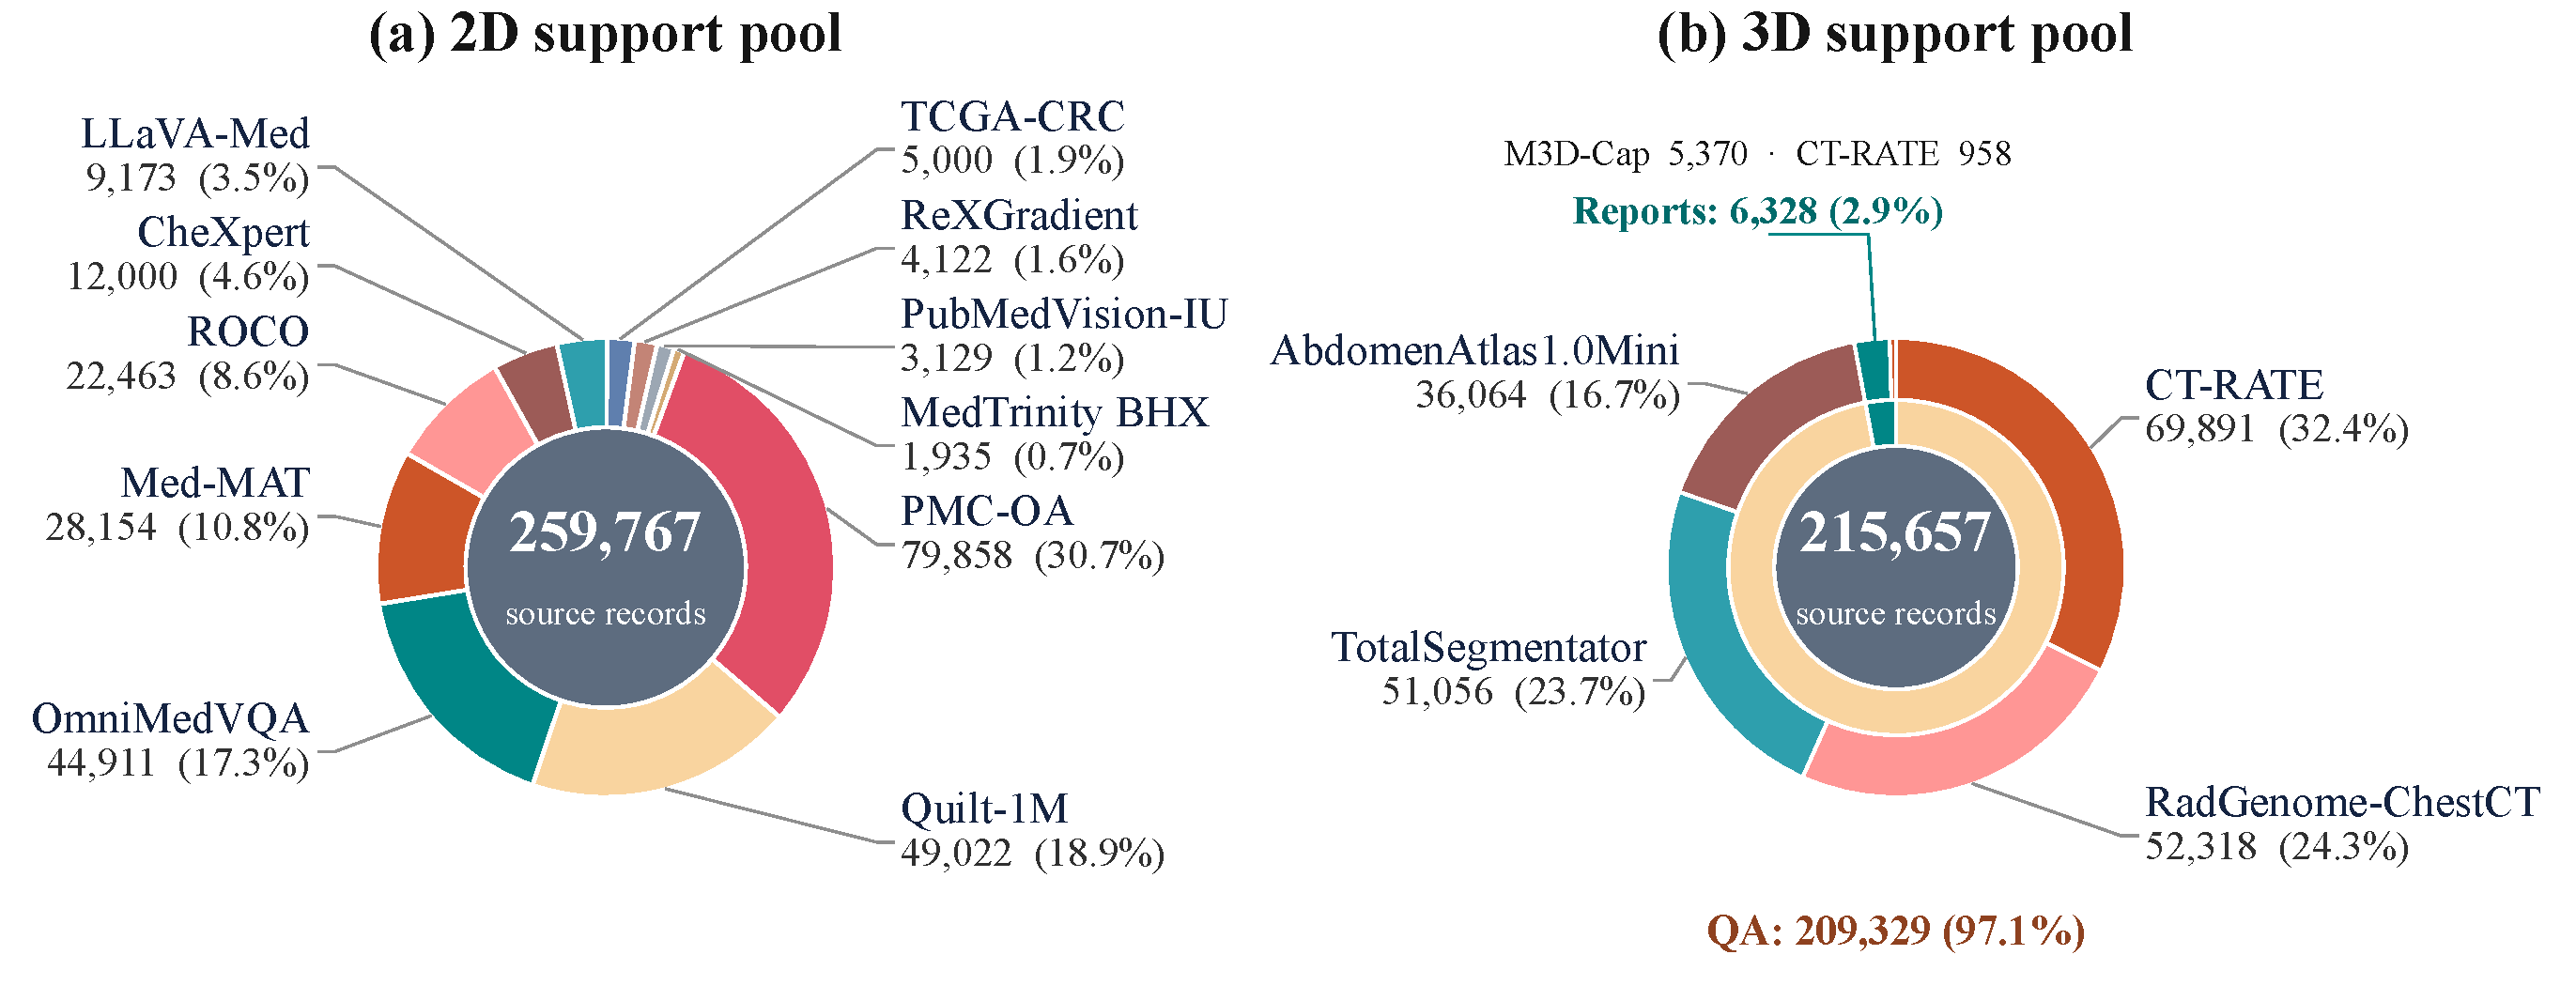
\includegraphics[width=\linewidth]{figures/support_composition.pdf}
\caption{支持集来源组成。（a）二维支持集包含259,767条源记录。（b）三维支持集包含215,657条源记录：内环区分问答与报告，外环表示相应来源。扇区面积与百分比均相对于各面板总量计算。}
\label{fig:support_composition}
\end{figure}

\begin{table}[!htbp]
\centering\small
\caption{支持集来源的官方资源。PubMedVision-IU、MedTrinity BHX 与 TCGA-CRC 的链接指向相应母数据集。}
\label{tab:support_links}
\setlength{\tabcolsep}{4pt}
\def\UrlFont{\footnotesize\sffamily}
\def\UrlBigBreaks{}
\begin{tabularx}{\linewidth}{@{}L{.28\linewidth}Y@{}}
\toprule
数据集 & 官方资源\\
\midrule
\multicolumn{2}{@{}l}{二维支持集}\\
PMC-OA\newline\citep{lin2023pmcclip} & \url{https://weixionglin.github.io/PMC-CLIP/}\\
Quilt-1M\newline\citep{ikezogwo2023quilt} & \url{https://github.com/wisdomikezogwo/quilt1m}\\
OmniMedVQA\newline\citep{hu2024omnimedvqa} & \url{https://github.com/OpenGVLab/Multi-Modality-Arena}\\
Med-MAT\newline\citep{cai2025medmat} & \url{https://github.com/FreedomIntelligence/Med-MAT}\\
ROCO\newline\citep{pelka2018roco} & \url{https://github.com/razorx89/roco-dataset}\\
CheXpert\newline\citep{irvin2019chexpert} & \url{https://aimi.stanford.edu/datasets/chexpert-chest-x-rays}\\
LLaVA-Med\newline\citep{li2023llava} & \url{https://github.com/microsoft/LLaVA-Med}\\
TCGA-CRC\newline\citep{tcga2012colorectal} & \url{https://gdc.cancer.gov/about-data/publications/coadread_2012}\\
ReXGradient\newline\citep{zhang2025rexgradient} & \url{https://huggingface.co/datasets/rajpurkarlab/ReXGradient-160K}\\
PubMedVision-IU 子集\newline\citep{chen2024pubmedvision} & \url{https://huggingface.co/datasets/FreedomIntelligence/PubMedVision}\\
MedTrinity BHX\newline\citep{xie2025medtrinity} & \url{https://github.com/UCSC-VLAA/MedTrinity-25M}\\
\midrule
\multicolumn{2}{@{}l}{三维支持集}\\
AbdomenAtlas1.0Mini\newline\citep{li2024abdomenatlas} & \url{https://huggingface.co/datasets/AbdomenAtlas/AbdomenAtlas1.0Mini}\\
CT-RATE\newline\citep{hamamci2026ctrate} & \url{https://huggingface.co/datasets/ibrahimhamamci/CT-RATE}\\
RadGenome-ChestCT\newline\citep{zhang2025radgenome} & \url{https://huggingface.co/datasets/RadGenome/RadGenome-ChestCT}\\
TotalSegmentator\newline\citep{wasserthal2023totalsegmentator} & \url{https://github.com/wasserth/TotalSegmentator}\\
M3D-Cap\newline\citep{bai2024m3d} & \url{https://huggingface.co/datasets/GoodBaiBai88/M3D-Cap}\\
\bottomrule
\end{tabularx}
\end{table}


% 根据作者更新的 数据加工.txt 整理；500 为目标规模，359,355 为事实数。
\begin{samepage}
\paragraph{源证据规范化与事实抽取。}
\label{app:data_preparation}
源数据加工将异质医学图文记录转化为可复用的事实证据，为学习者条件化的监督构造提供内容基础。每条记录保留视觉输入、原始文本与来源关联，报告样本保留同次检查的多幅影像。原生问答与分类标签通过规则转化为事实陈述，报告依据 Findings 与 Impression 分节组织，图像描述中的事实则由 Qwen3.6-27B 抽取。源记录沿任务形式、视觉能力、图像模态与解剖部位四个维度标注，使证据检索与课程指定的学习需求相对应。

质量控制考察记录的结构完整性、医学相关性与事实完备性，无有效事实的记录不参与监督构造。新增记录依据样本标识、影像路径及 RGB 像素内容去重，并检查与验证集影像的重合。最终源池提供359,355个可复用事实；该数量以事实条目计数，与图~\ref{fig:support_composition}中的源记录数量区分。

\par
\end{samepage}

\paragraph{基于任务的验证集构建。}
验证集以医学任务为基本组织单元，依据任务的输入属性与输出要求，对已有医学视觉问答与报告数据实施分层选样。问答任务按语言、答案类型、问题形式与内容类别分层，多项选择任务进一步考虑正确选项与问题长度；报告生成任务按影像数量等输入属性分层。各验证子集的目标规模统一设为500条，并保留样本标识、影像、问题及原始参考标注。由此形成的任务相关验证集合，用于持续估计学习者在不同任务条件下的能力表现及其学习响应。

\paragraph{基于任务的四维标注与能力诊断。}
四维标注依据医学任务的能力目标及其证据属性，表征验证实例所对应的任务条件（表~\ref{tab:feedback_axes}）。任务形式与视觉能力分别刻画输出结构与主要能力目标，图像模态与解剖部位则刻画任务所依托的医学证据。任务形式根据任务要求与答案格式确定；视觉问答实例的其余三维标签由 Qwen3.6-27B 依据影像、问题及参考答案补充，优先保留已有模态标注。胸部 X-ray 报告任务的四维标签依次为报告生成、整体描述、胸部 X-ray 与胸部。经格式与完整性检查后，依据这些任务属性分组汇总验证表现，刻画学习者在不同能力目标下的能力分布，为后续监督构造与课程分配确定任务重点。

\begin{table}[!htbp]
\centering\small
\caption{基于任务的验证集标注体系。任务形式与视觉能力刻画能力目标，图像模态与解剖部位刻画医学证据属性；各维度共同用于任务层面的能力诊断与课程适配。视觉能力维度包含九类。}
\label{tab:feedback_axes}
\setlength{\tabcolsep}{4pt}
\renewcommand{\arraystretch}{1.12}
\begin{tabularx}{\linewidth}{@{}lYY@{}}
\toprule
维度 & 类别或内容 & 标注依据\\
\midrule
任务形式 & 是非问答、开放短答、开放长答、多项选择、报告生成 & 任务要求与答案格式。\\
视觉能力 & 模态识别、器官识别、定位、空间关系、异常检测、属性判断、比较、整体描述、医学知识 & 问题的主要考查目标；报告任务归为整体描述。\\
图像模态 & CT、MRI、X-ray、超声、病理图像、论文图等 & 优先保留已有标注，缺失时由模型补充。\\
解剖部位或组织 & 胸部、腹部、脑、骨盆、四肢、脊柱及明确的器官或组织 & 影像与文本证据；无法确定时保留 unknown / other。\\
\bottomrule
\end{tabularx}
\end{table}


\subsection{评价指标与统计报告}

VQA 准确率依据预先确定的精确匹配或语义匹配准则计算。报告评价包含 BLEU-4、METEOR 和 ROUGE-L \citep{papineni2002bleu,banerjee2005meteor,lin2004rouge}。实现中的反馈复合指标为
$0.5\,\mathrm{ROUGE\mbox{-}L}+0.3\,\mathrm{BLEU\mbox{-}4}+0.2\,\mathrm{METEOR}$。
反馈分数 $U_t^{\mathrm{val}}$ 在 $\mathcal V_t$ 上计算，受控对照使用独立外部测试。图~\ref{fig:report_results}采用独立的医学报告评价指标 RaTEScore \citep{zhao2024ratescore}，乘以 100 展示。RaTEScore 不追溯替代用于课程分配的反馈分数。指标实现及精确/语义匹配选择须在受控对比前固定。实验一、二的结果与配对差值见表~\ref{tab:feedback_full}与表~\ref{tab:stage_full}。

纵向能力分析在比较前固定单元定义、$\mathcal V_t$ 内的样本面板、解码设置与越高越好的评分规则。在固定非空验证样本集合上计算$\mathcal J_c[M_e]$，报告样本数、单元内变化及修复/回退样本转移。不同任务采用与其目标相适应的评价指标刻画学习响应。第 $e$ 轮的独立验证反馈指导后续课程分配与构造原则的修订；外部基准用于评价各轮模型的学习结果，不参与课程决策。图~\ref{fig:trajectory}报告全部十轮记录，包括后续轮次的性能下降。稀疏单元标记为证据不足，不解释为能力变化。

\paragraph{检查点选择。}
\label{app:checkpoint_selection}
CoEvoMed-8B 的检查点选择依据医学问答与报告生成能力在不同训练轮次中的整体均衡性。R7 在所记录的十轮训练中呈现最为均衡的综合能力，因此六项二维主结果统一采用该检查点。使用同一检查点评价保留了同一学习者的联合能力表现；图~\ref{fig:trajectory}中各基准的单项峰值分别出现在 R7--R8。

\subsection{InternVL3-9B 跨骨干验证}
\label{app:internvl}

图~\ref{fig:internvl_trajectory}展示 InternVL3-9B 在 VQA-RAD 与 MIMIC-CXR 上的学习轨迹。两项任务分别训练独立模型，通过 LLaMA-Factory~\citep{zheng2024llamafactory}进行全参数监督微调，每轮从上一轮权重继续训练。曲线包含基线及全部八个已完成训练轮次。

VQA-RAD 准确率由56.98\%提高至第8轮的77.38\%，增加20.40个百分点，并在第6轮达到最高值78.71\%。MIMIC-CXR 的 RaTEScore 由50.55提高至63.83，增加13.28分，第4轮达到最高值65.34。两条轨迹在不同阶段达到峰值，最终轮次仍保留较大的性能增益。

\begin{figure}[H]
\centering
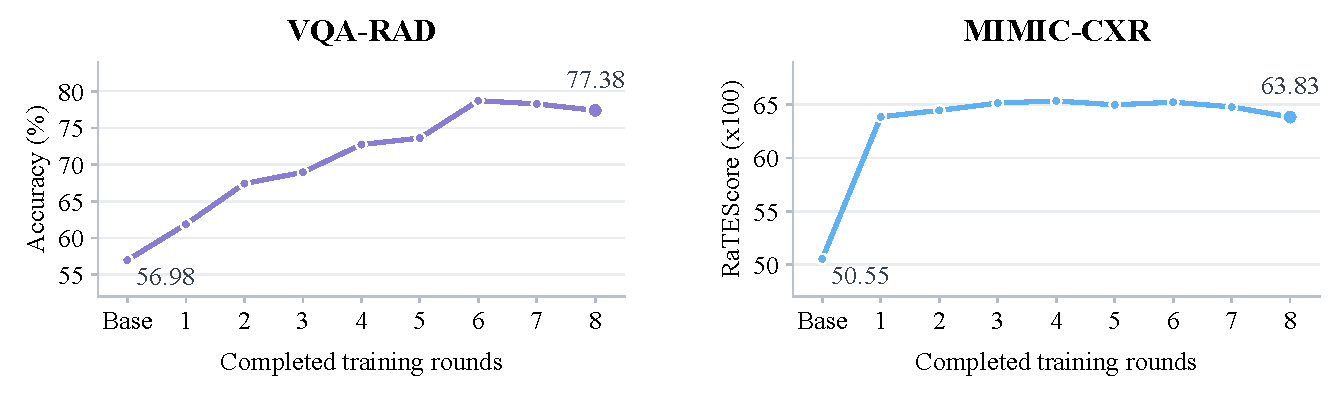
\includegraphics[width=\linewidth]{figures/internvl_trajectory.pdf}
\caption{InternVL3-9B 的学习轨迹。左：VQA-RAD 准确率（\%）；右：MIMIC-CXR RaTEScore，乘以100展示。两个面板对应分别训练的任务专用模型。Base 表示初始模型，1--8表示已完成训练轮次；仅标注基线与最后一轮数值。}
\label{fig:internvl_trajectory}
\end{figure}


\subsection{反馈来源与评价独立性}

CoEvoMed 使用独立于终测数据的任务验证集 $\mathcal V$。该验证集上的学习响应提供能力估计与课程回报，并指导构造原则的修订。外部基准集合 $\mathcal B_{\mathrm{ext}}$ 仅用于性能评价，不参与监督构造、学习者训练以及课程与原则更新。

\section{课程干预与组件对照}
\label{app:mechanisms}

\subsection{实验一：反馈与学习者状态的匹配性}
\label{app:feedback_ablation}

实验一将学习者初始状态固定为同一 R5 检查点，分别采用 R2、R3 的历史验证反馈与当前 R5 反馈。反馈由数值能力统计与错误语义摘要组成，前者刻画各任务的掌握水平与学习变化，后者概括尚未解决的错误模式。两部分共同替换为同一来源轮次的记录，用于指导课程分配与监督构造，以考察验证诊断与当前学习者状态的匹配性。表~\ref{tab:feedback_full}将正文表~\ref{tab:ablations}面板 A 扩展至六项二维基准，评测设置沿用附录~\ref{app:datasets_2d}。各组变化量均相对于同一 R5 进一步训练前的参照分数计算。R5 当前反馈组与实验二 D 组共用同一训练结果，对应图~\ref{fig:trajectory}中的第6轮。

\begin{table}[H]
\centering\scriptsize
\caption{固定 R5 学习者、共同替换数值能力统计与错误语义摘要的完整结果，反馈来源为 R2、R3 或 R5。VQA 为准确率（\%），报告生成为 RaTEScore（$\times100$）；括号内为相对 R5 进一步训练前的参照分数的变化。}
\label{tab:feedback_full}
\setlength{\tabcolsep}{3pt}
\renewcommand{\arraystretch}{1.18}
\begin{tabularx}{\linewidth}{@{}Yrrrrrr@{}}
\toprule
组别 & VQA-RAD & SLAKE & PMC-VQA & PathVQA & MIMIC-CXR & IU-Xray\\
\midrule
R5 训练前 & 73.61 & 89.00 & 64.60 & 65.80 & 59.00 & 61.63\\
R2 反馈 & 72.51 ($-1.10$) & 83.80 ($-5.20$) & 61.00 ($-3.60$) & 62.70 ($-3.10$) & 59.11 ($+0.11$) & 58.61 ($-3.02$)\\
R3 反馈 & 71.84 ($-1.77$) & 83.20 ($-5.80$) & 62.80 ($-1.80$) & 63.40 ($-2.40$) & 58.16 ($-0.84$) & 57.59 ($-4.04$)\\
\rowcolor{mainOurs} \textbf{R5 反馈} & 76.23 ($+2.62$) & 89.69 ($+0.69$) & 65.12 ($+0.52$) & 66.93 ($+1.13$) & 61.77 ($+2.77$) & 62.91 ($+1.28$)\\
\bottomrule
\end{tabularx}
\end{table}

当前 R5 反馈在六项基准上均优于历史反馈，并超过进一步训练前的参照分数：VQA-RAD 与 MIMIC-CXR 分别提高2.62个百分点与2.77分，SLAKE、PMC-VQA、PathVQA 与 IU-Xray 分别提高0.69、0.52、1.13和1.28分。R3 反馈在六项基准上均出现退化，R2 反馈仅在 MIMIC-CXR 上小幅提高，二者的相对排序随任务变化。这些结果支持同步更新数值与语义反馈，使后续课程干预适应学习者当前的能力状态与错误模式。

\subsection{实验二：监督构造原则的阶段依赖性}
\label{app:stage_transfer}

实验二将原始与演化构造原则分别用于完成第2轮（R2）和第5轮（R5）训练后的学习者。A、B 组从 R2 检查点出发，C、D 组从 R5 检查点出发，接受相应原则的训练干预。表~\ref{tab:stage_full}将正文表~\ref{tab:ablations}面板 B 扩展至六项基准，评测设置与实验一相同，变化量相对于各自阶段进一步训练前的参照分数计算。R5 参照与 D 组对应正文图~\ref{fig:trajectory}的第5轮与第6轮。

\begin{table}[H]
\centering\scriptsize
\caption{实验二在六项二维基准上的完整结果。括号内为相对对应阶段进一步训练前参照分数的变化。}
\label{tab:stage_full}
\setlength{\tabcolsep}{3pt}
\renewcommand{\arraystretch}{1.18}
\begin{tabularx}{\linewidth}{@{}Yrrrrrr@{}}
\toprule
组别 & VQA-RAD & SLAKE & PMC-VQA & PathVQA & MIMIC-CXR & IU-Xray\\
\midrule
R2 训练前 & 61.64 & 81.60 & 50.80 & 62.00 & 53.31 & 52.87\\
A: R2 / 原始 & 63.42 ($+1.78$) & 84.20 ($+2.60$) & 54.20 ($+3.40$) & 65.80 ($+3.80$) & 56.35 ($+3.04$) & 56.77 ($+3.90$)\\
B: R2 / 演化 & 59.20 ($-2.44$) & 81.00 ($-0.60$) & 48.00 ($-2.80$) & 65.40 ($+3.40$) & 56.47 ($+3.16$) & 56.69 ($+3.82$)\\
\midrule
R5 训练前 & 73.61 & 89.00 & 64.60 & 65.80 & 59.00 & 61.63\\
C: R5 / 原始 & 67.97 ($-5.64$) & 85.40 ($-3.60$) & 55.00 ($-9.60$) & 63.60 ($-2.20$) & 52.56 ($-6.44$) & 57.52 ($-4.11$)\\
\rowcolor{mainOurs} D: R5 / 演化 & 76.23 ($+2.62$) & 89.69 ($+0.69$) & 65.12 ($+0.52$) & 66.93 ($+1.13$) & 61.77 ($+2.77$) & 62.91 ($+1.28$)\\
\bottomrule
\end{tabularx}
\end{table}

四项 VQA 均呈现构造原则的排序反转：原始原则在 R2 上更优，演化原则在 R5 上更优。VQA-RAD 上，原始原则在 R2 领先4.22个百分点，演化原则在 R5 领先8.26个百分点；SLAKE、PMC-VQA 与 PathVQA 的演化减原始分差分别从$-3.20$、$-6.20$、$-0.40$变为$+4.29$、$+10.12$、$+3.33$个百分点。两项报告任务在 R2 上均受益于两种原则，原则间分差较小：MIMIC-CXR 上演化原则领先0.12分，IU-Xray 上原始原则领先0.08分；到 R5，演化原则分别领先9.21和5.39分。D 组在六项基准上均超过 R5 参照。这些结果表明，监督构造原则的效用随学习者阶段变化，支持依据学习响应持续修订监督。

\subsection{更大数据规模的原始数据训练对照}
\label{app:raw_source}

本对照考察增加原始数据量能否解释 CoEvoMed 的性能增益。两组从相同的 Qwen3-VL-8B 初始化出发，Qwen3+Raw 直接使用约 70 万条原始源数据训练，其训练样本量高于 CoEvoMed。该对照保留原始监督形式，不使用监督重构与自适应课程配置。两组均在附录~\ref{app:datasets_2d}中的四项 VQA 基准上进行评测。

\begin{table}[!htbp]
\centering\small
\caption{采用相同 Qwen3-VL-8B 初始化的医学 VQA 准确率（\%）。Qwen3+Raw 使用约 70 万条源数据，CoEvoMed 的训练样本量更少；初始模型作为参照。}
\label{tab:raw_source}
\setlength{\tabcolsep}{7pt}
\begin{tabular}{@{}lrrrr@{}}
\toprule
训练条件 & PMC-VQA & VQA-RAD & SLAKE & PathVQA\\
\midrule
Qwen3-VL-8B (base) & 54.13 & 56.76 & 64.84 & 42.77\\
Qwen3+Raw & 45.51 & 43.01 & 38.15 & 35.94\\
\rowcolor{mainOurs} CoEvoMed-8B & \textbf{67.95} & \textbf{82.48} & \textbf{91.60} & \textbf{69.40}\\
\bottomrule
\end{tabular}
\end{table}

CoEvoMed 以更少的训练数据，在 PMC-VQA、VQA-RAD、SLAKE 与 PathVQA 上分别较 Qwen3+Raw 提升 22.44、39.47、53.45 与 33.46 个百分点。原始源数据直接训练在四项基准上均低于初始模型，而 CoEvoMed 均取得提升。因此，扩大原始数据规模未能复现 CoEvoMed 的性能增益。这些结果支持学习响应驱动的监督构造与课程适配的有效性：将源证据转化为契合学习者动态需求的监督，能够提高训练数据的学习价值。

\section{形式化的适用范围}
\label{sec:limitations}

课程构造映射是随机的学习者条件化转换。经验生成与分配通过训练影响能力发展，从而塑造学习轨迹。有限验证样本提供部分能力证据，各能力单元保留自身评分尺度；独立外部测试评价重复使用验证反馈后的泛化表现。

局部干预提供被测学习者状态与构造版本上的证据。适用性论断以被评价的数据与骨干协议为范围；医学基准表现及源证据验证不等同于临床安全性或患者获益。

\section{完整形式化模型与符号说明}
\label{app:formalization}

本附录形式化第~\ref{sec:problem}节所述的共演化。学习者$M_e$与智能体的构造原则$\Sigma_e$构成完整状态$X_e$中相互依赖的两个部分。式~\ref{eq:construction}中的映射$\mathfrak C_e$结合分配、生效原则与证据验证形成学习者更新所需的监督。更新后的响应进入历史并引导原则修订，$\Phi(h_e)$提供分配策略输入。固定的$\mathcal J_c$评价各轮能力，形成$E$轮训练的能力轨迹$\Gamma_E=(\widehat{\boldsymbol\kappa}_0,\ldots,\widehat{\boldsymbol\kappa}_E)$，分配策略在这一耦合动态中优化累积验证进展。

\subsection{能力分布与验证观测}

式~\ref{eq:capability_level}以能力评价泛函$\mathcal J_c$将学习者在固定验证集上的预测行为映射为标量能力坐标，定义实测掌握水平$\mathcal J_c[M_e]$。该泛函由固定验证集$\mathcal V_c$及实例评价规则$u_c$确定。每个$\mathcal V_c$属于相应任务验证集$\mathcal V_t$，在比较前确定样本身份、评分规则与解码设置。式~\ref{eq:capability_change}以同一泛函在相邻轮次学习者上的取值之差衡量学习进展，等价于对同一集合逐样本计算评价变化后取平均。初始评估提供掌握水平；缺失观测单独标记。

VQA反馈记录修复与回退的样本。报告反馈在$\mathcal V_t$上跟踪分数变化与持续低分情况；报告缺口采用固定低分标准，而非用1减去复合分数。反馈摘要保留当前表现、相邻轮次的变化、能力缺口与既往资源分配。

以$o_e$表示第$e$轮验证观测，包括测量表现与错误证据。可观测交互历史为
\[
h_e=(o_0,a_0,r_0,\ldots,a_{e-1},r_{e-1},o_e),
\qquad \mathbf{s}_e=\Phi(h_e).
\]
其中，$a_e$为课程动作，$r_e$为式~\ref{eq:gain}定义的奖励，$\Phi$将交互历史压缩为规划器输入。第$e$轮使用$\Sigma_e$构造监督并更新学习者，随后将$a_e,r_e,o_{e+1}$加入历史。式~\ref{eq:strategy_evolution}依据所得$h_{e+1}$修订原则，更新后的$\Sigma_{e+1}$供下一轮使用。课程规划器依据历史摘要决策，完整状态转移定义在$X_e$上。

\subsection{完整状态与部分可观测动态}

对于预先规定的构造原则演化规则$\mathscr E$，有限时域过程为
\[
\mathcal M_{\mathscr E}=(\mathcal X,\mathcal A_{\mathrm{act}},\mathcal O,P_{\mathscr E},\Omega,R,\rho_0,\gamma,E).
\]
$\mathcal X$、$\mathcal A_{\mathrm{act}}$与$\mathcal O$分别表示完整系统状态、允许的课程动作及验证观测所在的空间。$P_{\mathscr E}$描述包含构造原则更新的状态转移，$\Omega$描述给定完整状态时的观测分布。奖励规则$R$产生式~\ref{eq:gain}~中的奖励；$\rho_0$为初始状态分布，$\gamma$为折扣因子，$E$为决策轮数。

状态$X_e\in\mathcal X$包含学习者参数与训练状态、当前构造原则、保留的训练数据、反馈与演化统计、调度信息以及剩余资源。状态保留固定运行规则下后续更新所需的信息。
式~\ref{eq:transition}给出正文采用的马尔可夫状态转移。
初始化与观测分别满足$X_0\sim\rho_0$和$o_e\sim\Omega(\cdot\mid X_e)$。训练引起的能力变化发生在状态转移内部，无需假设该完整状态上的转移核随时间改变。数据构造、筛选、学习者优化以及计划内的构造原则更新共同构成转移。实现中的一个 episode 对应一个决策步，而非完整的 POMDP 轨迹。

\subsection{训练分布与资源约束}

第~\ref{sec:multiagent}节中的多智能体角色共同实现随机的课程构造映射
\begin{equation}
\mathcal D_e^{\mathrm{syn}}=\mathfrak C_e(\mathcal S,h_e),
\qquad
\mathfrak C_e=\mathfrak C[\mu_{\theta_e},\Sigma_e].
\label{eq:construction}
\end{equation}
该映射结合策略引导的分配、原则约束的生成与证据一致性验证，所得监督进入式~\ref{eq:learning_dynamics}的训练混合。式~\ref{eq:supervision_mixture}刻画验证前候选样本的分布，下标$e$包含对当前历史$h_e$与课程动作$a_e$的依赖。

令$z=(v,x,y)$表示由视觉输入、指令与目标回答组成的构造样本。给定反馈$\mathbf{s}_e$，采样动作$a_e\sim\mu_\theta(\cdot\mid \mathbf{s}_e)$通过分配映射确定各能力单元的候选样本配额份额$q_{e,c}$。条件构造器$g_{\Sigma_e}$规定使用当前构造原则与支持证据生成样本的方式。质量筛选前，二者的共同作用可分解为
\begin{equation}
p_e(z,c\mid h_e,a_e,\Sigma_e)
=q_{e,c}\,
g_{\Sigma_e}(z\mid c,\mathcal S,h_e,a_e).
\label{eq:factorization}
\end{equation}
对$c$求边缘分布可得式~\ref{eq:supervision_mixture}，其中$g_{e,c}(z;\Sigma_e,\mathcal S)=g_{\Sigma_e}(z\mid c,\mathcal S,h_e,a_e)$。$q_{e,c}$在候选数据分布中充当混合权重，在$\mathcal C$上的总和为1，并满足式~\ref{eq:quota}。该分解描述按候选配额抽取一条记录的边缘分布，批内生成可以相互依赖。质量筛选改变接受样本及其比例；实际训练曝光还取决于原始或回放数据的混合与训练采样。候选数、接受数、训练 token 及模型调用成本分别核算。

构造原则$\Sigma_e$与份额$\boldsymbol q_e$分别控制候选监督的内容与能力间构成，筛选及混合协议进一步决定训练分布。学习者采用式~\ref{eq:student}的回答 token 损失进行优化，课程分配通过 PPO 学习，原则修订比较基于相同医学证据生成的样本（第~\ref{sec:strategy_evolution}节）。固定的验证评价准则$\mathcal J_c$记录所得能力变化，为后续适应提供学习响应。

式~\ref{eq:objective}~中的简写目标将策略搜索限制在满足预算的范围内。显式写出初始化与转移依赖，可得
\begin{equation}
\begin{aligned}
\max_{\pi\in\Pi_{\mathrm{adm}}}\quad&
\E_{\rho_0,\pi,P_{\mathscr E},\Omega}
\left[\sum_{e=0}^{E-1}\gamma^e r_e\right]\\
\text{subject to}\quad&
\sum_{e=0}^{E-1}\mathbf k_e\preceq\mathbf B ,
\end{aligned}
\label{eq:objective_full}
\end{equation}
其中，$\Pi_{\mathrm{adm}}$表示满足课程动作与分配配额约束的策略集合。向量$\mathbf k_e$记录第$e$轮资源消耗，$\mathbf B$给出各类资源的总预算，$\preceq$表示逐分量满足预算约束。期望涵盖固定运行协议下随机的课程动作、数据构造与学习者更新。

规定的构造原则演化规则参与状态转移并影响后续学习回报，PPO 优化分配策略。奖励等于相邻模型之间的验证增益，对 VQA 与报告生成赋予相同权重，同时保留改善与回退。独立外部测试另行评价所得泛化表现，与折扣训练回报分别报告。

\subsection{累积增益与学习过程的关系}
\label{app:cumulative_gains}

采用式~\ref{eq:gain}中固定的任务族权重与评分尺度，定义
\[
F_e=\frac{1}{2|\mathcal T_{\mathrm V}|}\sum_{t\in\mathcal T_{\mathrm V}}U_t^{\mathrm{val}}(M_e)
+\frac{1}{2|\mathcal T_{\mathrm R}|}\sum_{t\in\mathcal T_{\mathrm R}}U_t^{\mathrm{val}}(M_e).
\]
于是$r_e=F_{e+1}-F_e$。对于固定时域$E\geq1$及$0<\gamma\leq1$，移动求和下标可得
\begin{equation}
\begin{aligned}
\sum_{e=0}^{E-1}\gamma^e(F_{e+1}-F_e)
&=\sum_{e=1}^{E}\gamma^{e-1}F_e-\sum_{e=0}^{E-1}\gamma^eF_e\\
&=-F_0+(1-\gamma)\sum_{e=1}^{E-1}\gamma^{e-1}F_e+\gamma^{E-1}F_E.
\end{aligned}
\label{eq:trajectory_objective}
\end{equation}
该恒等式对每条交互轨迹成立，取期望后即得到式~\ref{eq:objective}的等价目标。固定初始学习者使$F_0$为常数；$\gamma<1$赋予中间阶段及终点表现非负权重，$\gamma=1$时中间项抵消。这里的标量目标聚合任务表现，能力轨迹$\Gamma_E$保留单元级变化。

\clearpage
\section{对话案例展示}
\label{app:showcase}

图~\ref{fig:showcase_path_pmc}--\ref{fig:showcase_m3d}展示 CoEvoMed 对话案例，覆盖六个二维与三个三维基准。每个区块呈现视觉输入、用户问题与模型回答，GT 表示参考答案。

\begin{figure}[H]
\centering
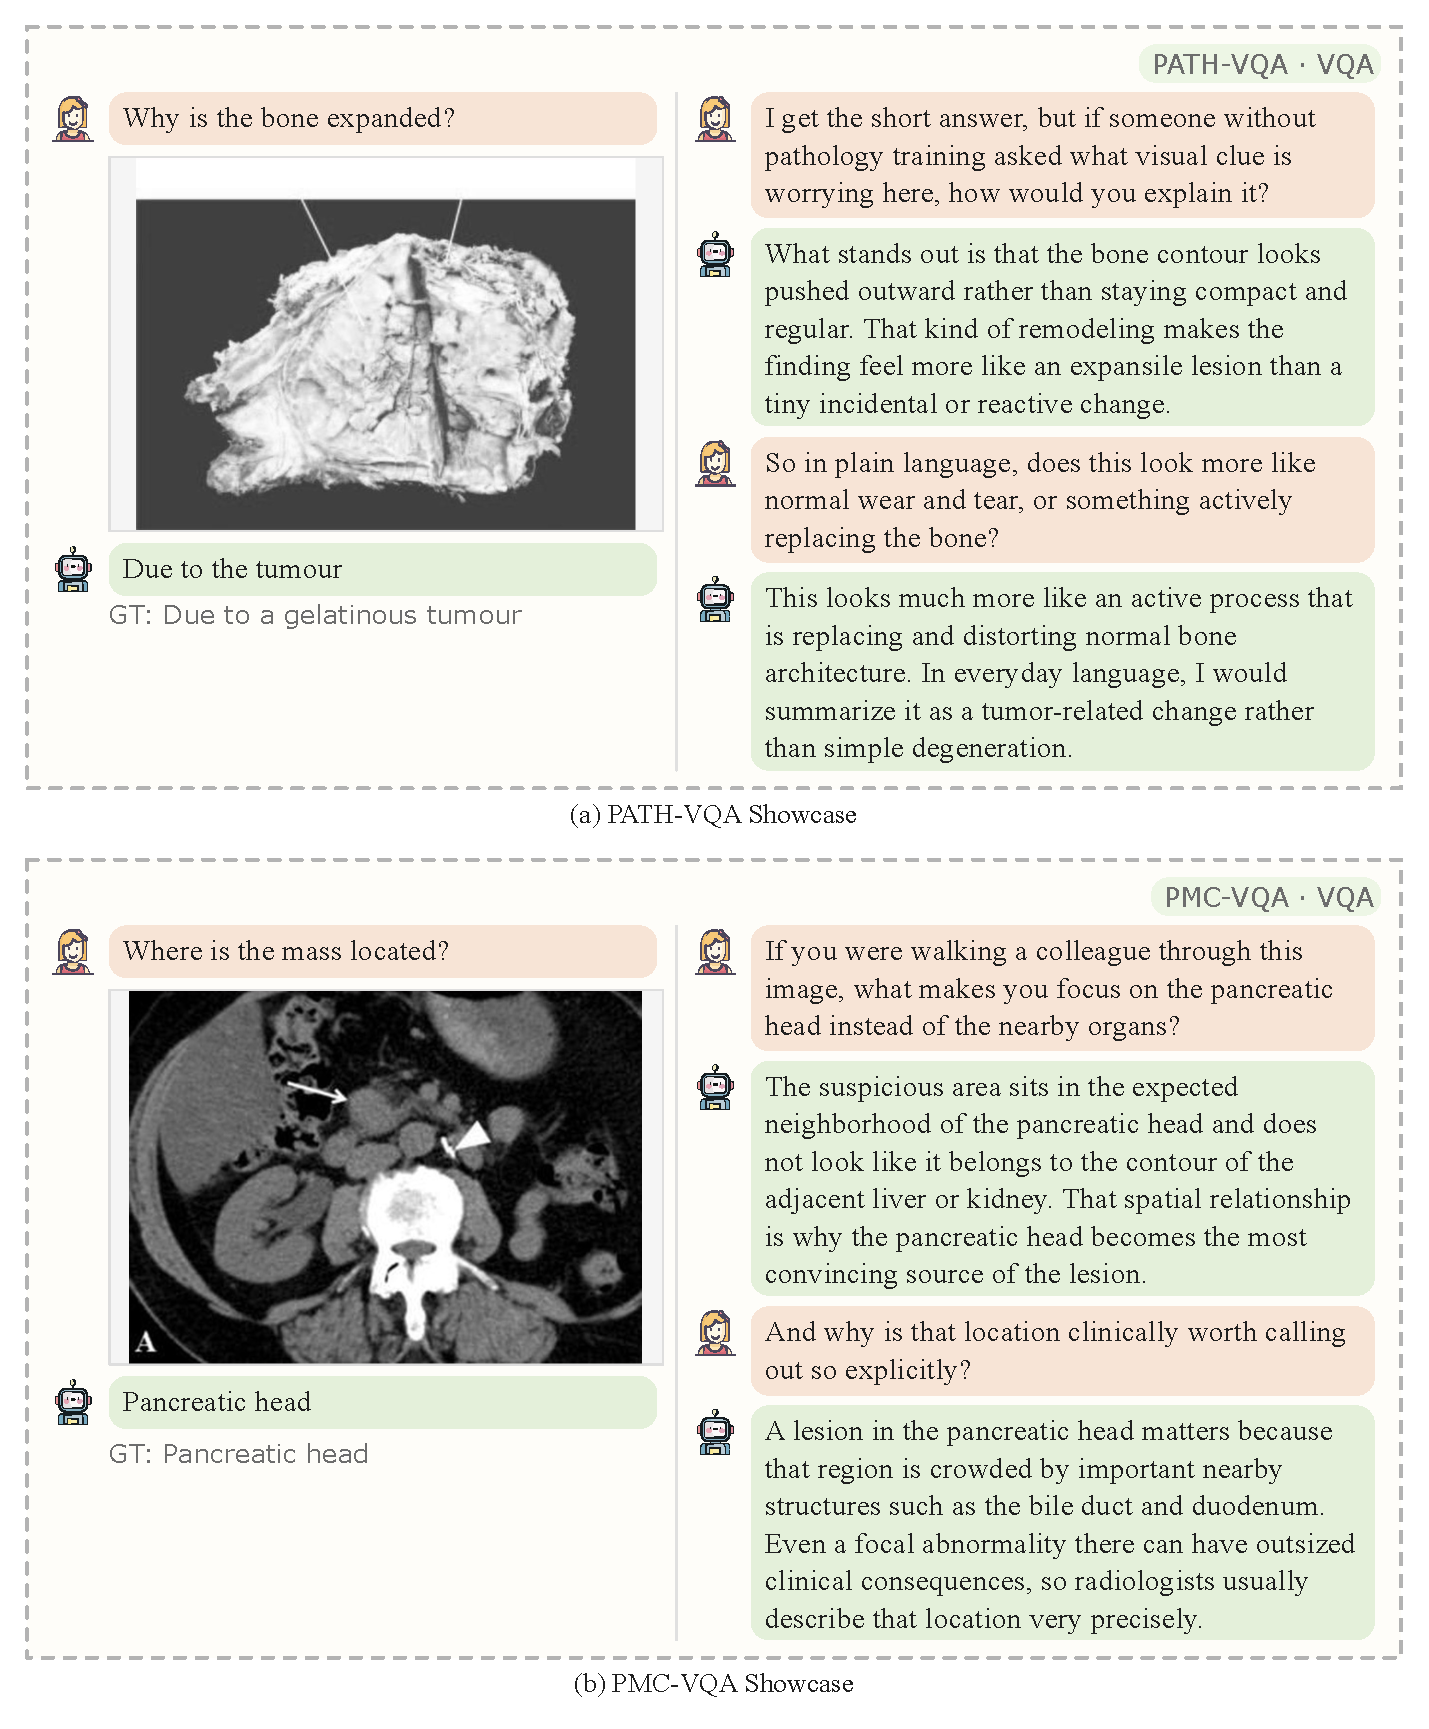
\includegraphics[width=\linewidth]{figures/showcase/medical_vqa_2d.pdf}
\caption{CoEvoMed 在 PathVQA（上）与 PMC-VQA（下）的多轮对话案例。}
\label{fig:showcase_path_pmc}
\end{figure}

\clearpage
\begin{figure}[H]
\centering
\includegraphics[page=2,width=\linewidth]{figures/showcase/medical_vqa_2d.pdf}
\caption{CoEvoMed 在 SLAKE（上）与 VQA-RAD（下）的多轮对话案例。}
\label{fig:showcase_slake_rad}
\end{figure}

\clearpage
\begin{figure}[H]
\centering
\includegraphics[page=3,width=\linewidth]{figures/showcase/medical_vqa_2d.pdf}
\caption{CoEvoMed 在 IU-Xray（上）与 MIMIC-CXR（下）的报告生成多轮对话案例。}
\label{fig:showcase_reports}
\end{figure}

\clearpage
\begin{figure}[H]
\centering
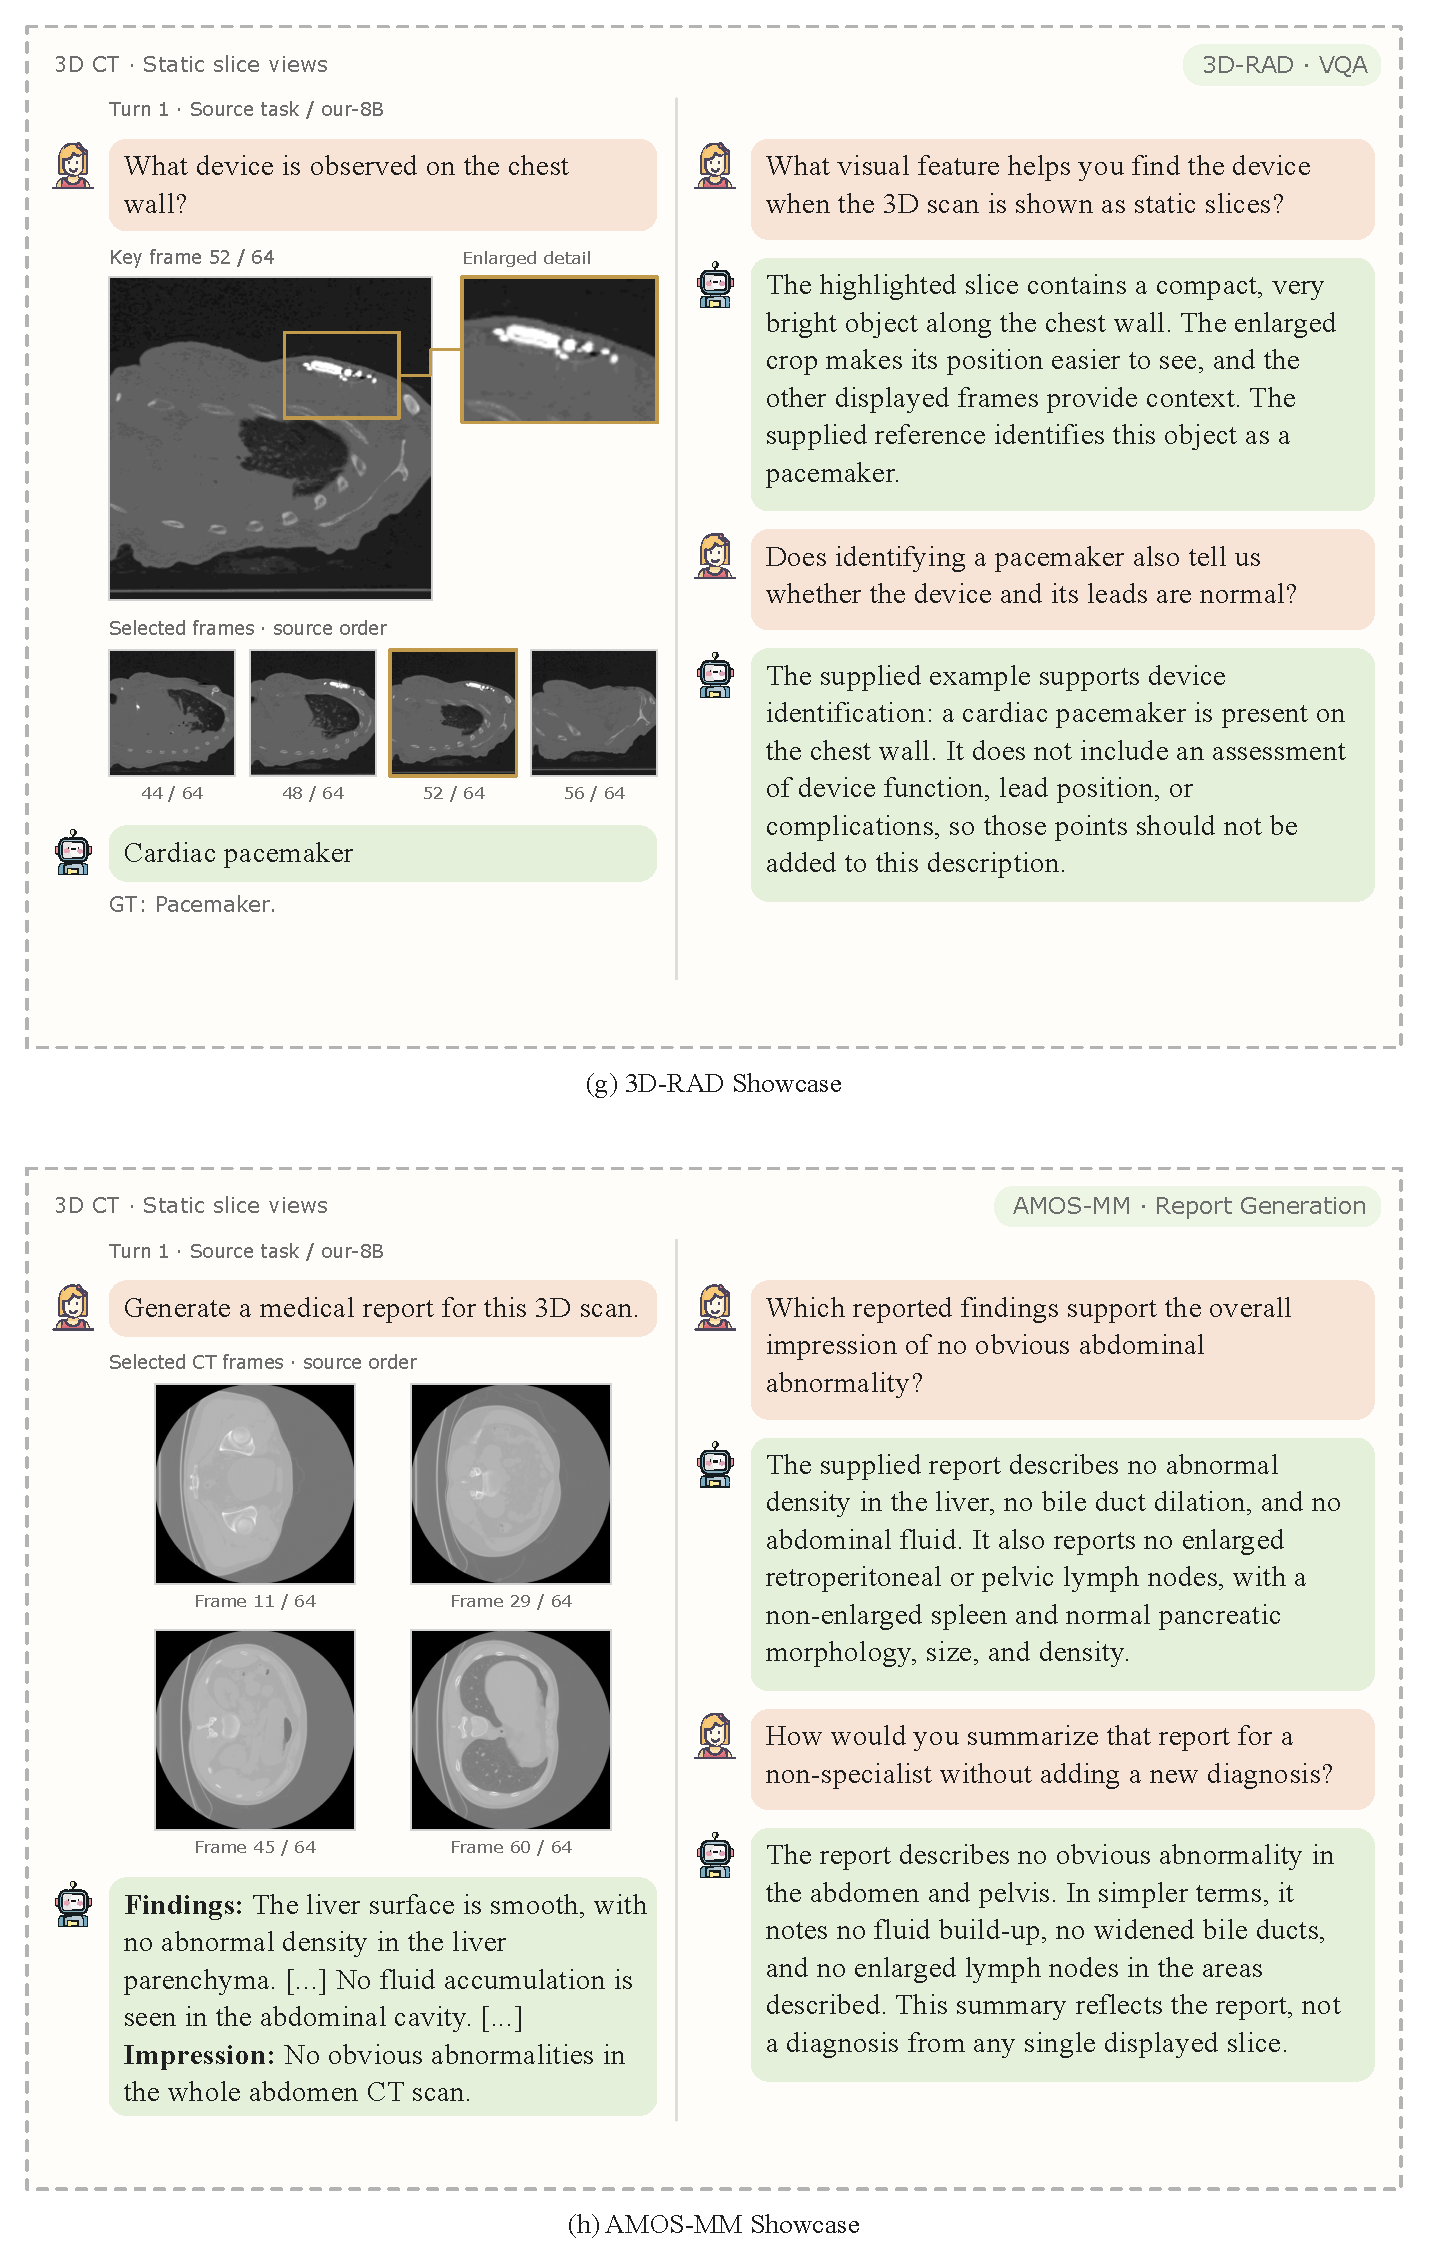
\includegraphics[width=\linewidth,height=0.86\textheight,keepaspectratio]{figures/showcase/medical_vqa_3d_pairs.pdf}
\caption{CoEvoMed 在 3D-RAD（上）与 AMOS-MM（下）的多轮对话案例及选定 CT 切片。AMOS-MM 报告以节选形式展示，省略号标记省略内容。}
\label{fig:showcase_rad_amos}
\end{figure}

\clearpage
\begin{figure}[H]
\centering
\includegraphics[page=2,width=\linewidth]{figures/showcase/medical_vqa_3d_pairs.pdf}
\caption{CoEvoMed 在 M3D-VQA 上的多轮对话案例、选定 CT 切片及局部放大图。}
\label{fig:showcase_m3d}
\end{figure}


\end{document}
